% This is the main LaTeX file which is used to produce the Biopython
% Tutorial documentation.
%
% If you just want to read the documentation, you can pick up ready-to-go 
% copies in both pdf and html format from:
%
% http://www.biopython.org/documentation/
%
% If you want to typeset the documentation, you'll need a standard TeX/LaTeX
% distribution (I use teTeX, which works great for me on unix platforms).
% Additionally, you need HeVeA (or at least hevea.sty), which can be
% found at:
%
% http://pauillac.inria.fr/~maranget/hevea/index.html
% 
% You will also need the pictures included in the document, which are
% UMLish diagrams created by Dia 
% (http://www.lysator.liu.se/~alla/dia/dia.html).
% These diagrams are available from biopython CVS in the original dia 
% format, which you can easily save as .png format using Dia itself.
% They are also checked in as the png files, so if you make
% modifications to the original dia files, the png files should also be
% changed.
%
% Once you're all set, you should be able to generate pdf by running:
% 
% pdflatex Tutorial.tex  (to generate the first draft)
% pdflatex Tutorial.tex  (to get the cross references right)
% pdflatex Tutorial.tex  (to get the table of contents right) 
%
% To generate the html, you'll need HeVeA installed. First, remove the
% Tutorial.aux file generated by LaTeX, then run:
% 
% hevea -fix Tutorial.tex   (to generate the html file)
% hevea -fix Tutorial.tex   (to get the references correct)
% hacha Tutorial.html  (to split the html file into sections)
%
% If you want to typeset this and have problems, please report them
% at biopython-dev@biopython.org, and we'll try to get things resolved. We 
% always love to have people interested in the documentation!

\documentclass{report}
\usepackage{url}
\usepackage{fullpage}
\usepackage{hevea}
\usepackage{graphicx}

% make everything have section numbers
\setcounter{secnumdepth}{4}

% Make links between references
\usepackage{hyperref}
\newif\ifpdf
\ifx\pdfoutput\undefined
  \pdffalse
\else
  \pdfoutput=1
  \pdftrue
\fi
\ifpdf
  \hypersetup{colorlinks=true, hyperindex=true, citecolor=red, urlcolor=blue}
\fi

\begin{document}

\title{Biopython Tutorial and Cookbook}
\author{Jeff Chang, Brad Chapman, Iddo Friedberg, Thomas Hamelryck}
\date{Last Update--16 Feb 2005}

\maketitle
\tableofcontents

\chapter{Introduction}

\section{What is Biopython?}

The Biopython Project is an international association of developers of freely available Python (\ahrefurl{\url{http://www.python.org}}) tools for computational molecular biology. The web site \ahrefurl{\url{http://www.biopython.org}} provides an online resource for modules, scripts, and web links for developers of Python-based software for life science research.


Basically, we just like to program in python and want to make it as easy as possible to use python for bioinformatics by creating high-quality, reusable modules and scripts.

\subsection{What can I find in the Biopython package}

The main Biopython releases have lots of functionality, including:

\begin{itemize}
  \item The ability to parse bioinformatics files into python utilizable data structures, including support for the following formats:

  \begin{itemize}
    \item Blast output -- both from standalone and WWW Blast
    \item Clustalw
    \item FASTA
    \item GenBank
    \item PubMed and Medline
    \item Expasy files, like Enzyme, Prodoc and Prosite
    \item SCOP, including 'dom' and 'lin' files
    \item Rebase
    \item UniGene
    \item SwissProt
  \end{itemize}

  \item Files in the supported formats can be iterated over record by record or indexed and accessed via a Dictionary interface.

  \item Code to deal with popular on-line bioinformatics destinations such as:

  \begin{itemize}
    \item NCBI -- Blast, Entrez and PubMed services
    \item Expasy -- Prodoc and Prosite entries
  \end{itemize}

  \item Interfaces to common bioinformatics programs such as:

  \begin{itemize}
    \item Standalone Blast from NCBI
    \item Clustalw alignment program.
  \end{itemize}

  \item A standard sequence class that deals with sequences, ids on sequences, and sequence features.

  \item Tools for performing common operations on sequences, such as translation, transcription and weight calculations.

  \item Code to perform classification of data using k Nearest Neighbors, Naive Bayes or Support Vector Machines.

  \item Code for dealing with alignments, including a standard way to create and deal with substitution matrices.

  \item Code making it easy to split up parallelizable tasks into separate processes.

  \item GUI-based programs to do basic sequence manipulations, translations, BLASTing, etc.

  \item Extensive documentation and help with using the modules, including this file, on-line wiki documentation, the web site, and the mailing list.

  \item Integration with other languages, including the Bioperl and Biojava projects, using the BioCorba interface standard (available with the biopython-corba module).

\end{itemize}

We hope this gives you plenty of reasons to download and start using Biopython!

\section{Installing Biopython}

All of the installation information for Biopython was separated from
this document to make it easier to keep updated. The instructions cover
installation of python, Biopython dependencies and Biopython itself.
It is available in pdf
(\ahrefurl{\url{http://www.biopython.org/docs/install/Installation.pdf}})
and html formats
(\ahrefurl{\url{http://www.biopython.org/docs/install/Installation.html}}).

\section{FAQ}

\begin{enumerate}
  \item \emph{I looked in a directory for code, but I couldn't seem to find the code that does something. Where's it hidden?} \\
  One thing to know is that we put code in \verb|__init__.py| files. If you are not used to looking for code in this file this can be confusing. The reason we do this is to make the imports easier for users. For instance, instead of having to do a ``repetitive'' import like \verb|from Bio.GenBank import GenBank|, you can just import like \verb|from Bio import GenBank|.

  \item \emph{What happened to the} \verb|br_regrtest.py| \emph{regression tests?}
  We updated the regression testing framework to use PyUnit, and also to fix newline problems. \verb|br_regrtest.py| is still there, but almost all of its functionality has been moved (well, copy and pasted) to \verb|run_tests.py|.

  \item \emph{Why do some of the tests fail when running the regression tests with output like}: \\
\verb|Writing: '\012', expected: '\015'| \\
 This shouldn't happen any more! We updated the regression testing suite so that it uses PyUnit and we hopefully have fixed newline problems. Please let us know if any tests fail.
\end{enumerate}

\chapter{Quick Start -- What can you do with Biopython?}

This section is designed to get you started quickly with Biopython, and to give a general overview of what is available and how to use it. All of the examples in this section assume that you have some general working knowledge of python, and that you have successfully installed Biopython on your system. If you think you need to brush up on your python, the main python web site provides quite a bit of free documentation to get started with (\ahrefurl{\url{http://www.python.org/doc/}}). 

 
Since much biological work on the computer involves connecting with databases on the internet, some of the examples will also require a working internet connection in order to run. 


Now that that is all out of the way, let's get into what we can do with Biopython.

\section{General overview of what Biopython provides}

As mentioned in the introduction, Biopython is a set of libraries to provide the ability to deal with ''things'' of interest to biologists working on the computer. In general this means that you will need to have at least some programming experience (in python, of course!) or at least an interest in learning to program. Biopython's job is to make your job easier as a programmer by supplying reusable libraries so that you can focus on answering your specific question of interest, instead of focusing on the internals of parsing a particular file format (of course, if you want to help by writing a parser that doesn't exist and contributing it to Biopython, please go ahead!). So Biopython's job is to make you happy!


One thing to note about Biopython is that it often provides multiple ways of ``doing the same thing.'' To me, this can be frustrating since I often way to just know the one right way to do something. However, this is also a real benefit because it gives you lots of flexibility and control over the libraries. The tutorial helps to show you the common or easy ways to do things so that you can just make things work. To learn more about the alternative possibilities, look into the Cookbook section (which tells you some cools tricks and tips) and the Advanced section (which provides you with as much detail as you'd ever want to know!). 

\section{Working with sequences}
\label{sec:sequences}

Disputedly (of course!), the central object in bioinformatics is the sequence. Thus, we'll start with the Biopython mechanisms for dealing with sequences. When I think of a sequence the first thing that pops into my mind is a string of letters:\verb| 'AGTACACTGGT'| which seems natural since this is the most common way that sequences are seen in biological file formats.  However, a simple string of letters by itself is also very uninformative -- is it a DNA or  protein sequence (okay, a protein with a lot of Alanines, Glycines, Cysteines and Threonines!), what type of organism did it come from, what is so interesting about it, and so on. The challenge in designing a sequence interface is to pick a representation that is informative enough to take into account the more complex information, yet is as lightweight and easy to work with as just a simple sequence.


The approach taken in the Biopython sequence class is to utilize a class that holds more complex information, yet can be manipulated as if it were a simple string. This is accomplished by utilizing operator overloading to make manipulating a sequence object feel like manipulating a python string. The sequence class, referred to simply as Seq,  is defined in the file \verb|Bio/Seq.py.| Let's look at the Seq class deeper to see what it has to offer.


A biopython Seq object has two important attributes:

\begin{enumerate}

\item \verb|data| -- as the name implies, this is the actual sequence data string of the sequence.

\item \verb|alphabet| -- an object describing what the individual characters making up the string ``mean'' and how they should be interpreted.

\end{enumerate}

Clearly the alphabet object is the important thing that is making the Seq object more than just a string. The currently available alphabets for Biopython are defined in the \verb|Bio/Alphabet| module. We'll use the IUPAC alphabets \ahrefurl ({\url{http://www.chem.qmw.ac.uk/iupac/}}) here to deal with some of our favorite objects: DNA, RNA and Proteins.  


\verb|Bio/Alphabet/IUPAC.py| provides basic definitions for proteins, DNA and RNA, but additionally provides the ability to extend and customize the basic definitions. For instance, for proteins, there is a basic IUPACProtein class, but there is an additional ExtendedIUPACProtein class providing for the additional elements ``Asx'' (asparagine or aspartic acid), ``Sec'' (selenocysteine), and ``Glx'' (glutamine or glutamic acid). For DNA you've got choices of IUPACUnambiguousDNA, which provides for just the basic letters, IUPACAmbiguousDNA (which provides for ambiguity letters for every possible situation) and ExtendedIUPACDNA, which allows letters for modified bases. Similarly, RNA can be represented by IUPACAmbigousRNA or IUPACUnambigousRNA.


The advantages of having an alphabet class are two fold. First, this gives an idea of the type of information the \verb|data| object contains. Secondly, this provides a means of constraining the information you have in the data object, as a means of type checking.


Now that we know what we are dealing with, let's look at how to utilize this class to do interesting work.


First, create a Sequence object from a string of information we've got. We'll create an unambiguous DNA object:

\begin{verbatim}
>>> from Bio.Alphabet import IUPAC
>>> my_alpha = IUPAC.unambiguous_dna
>>> from Bio.Seq import Seq
>>> my_seq = Seq('GATCGATGGGCCTATATAGGATCGAAAATCGC', my_alpha)
>>> print my_seq
Seq('GATCGATGGGCCTATATAGGATCGAAAATCGC', IUPACUnambiguousDNA())
\end{verbatim}


Even though this is a sequence object, we can deal with it in some ways as if it were a normal python string. For instance, let's get a slice of the sequence.

\begin{verbatim}
>>> my_seq[4:12]
Seq('GATGGGCC', IUPACUnambiguousDNA())
\end{verbatim}

Two things are interesting to note. First, this follows the normal conventions for python sequences.  So the first element of the sequence is 0 (which is normal for computer science, but not so normal for biology). When you do a slice the first item is included (i.~e.~4 in this case) and the last is excluded (12 in this case), which is the way things work in python, but of course not necessarily the way everyone in the world would expect. The main goal is to stay consistent with what python does. The second thing to notice is that the slice is performed on the sequence data string, but the new object produced retains the alphabet information from the original Seq object.


You can treat the Seq object like the string in many ways:

\begin{verbatim}
>>> len(my_seq)
32
>>> new_seq = my_seq[0:5]
>>> print new_seq
Seq('GATCG', IUPACUnambiguousDNA())
>>> my_seq + new_seq
Seq('GATCGATGGGCCTATATAGGATCGAAAATCGCGATCG', IUPACUnambiguousDNA())
>>> my_seq[5]
'A'
>>> my_seq == new_seq
0
\end{verbatim}

In all of the operations, the alphabet property is maintained. This is very useful in case you accidentally end up trying to do something weird like add a protein sequence and a DNA sequence:

\begin{verbatim}
>>> protein_seq = Seq('EVRNAK', IUPAC.protein)
>>> dna_seq = Seq('ACGT', IUPAC.unambiguous_dna)
>>> protein_seq + dna_seq
Traceback (most recent call last):
  File "<stdin>", line 1, in ?
  File "/usr/local/lib/python1.6/site-packages/Bio/Seq.py", line 42, in __add__
    raise TypeError, ("incompatable alphabets", str(self.alphabet),
TypeError: ('incompatable alphabets', 'IUPACProtein()', 'IUPACUnambiguousDNA()')
\end{verbatim}


And if you are really just need the string to insert into something, this is very easy to extract:

\begin{verbatim}
>>> my_seq.tostring()
'GATCGATGGGCCTATATAGGATCGAAAATCGC'
\end{verbatim} 

The sequence object is not mutable by default, since in many biological applications you want to ensure you are not changing your data:

\begin{verbatim}
>>> my_seq[5] = 'G'
Traceback (most recent call last):
  File "<stdin>", line 1, in ?
AttributeError: 'Seq' instance has no attribute '__setitem__'
\end{verbatim}

However, you can convert it into a mutable sequence and do pretty much anything you want with it:

\begin{verbatim}
>>> mutable_seq = my_seq.tomutable()
>>> print mutable_seq
MutableSeq('GATCGATGGGCCTATATAGGATCGAAAATCGC', IUPACUnambiguousDNA())
>>> mutable_seq[5] = 'T'
>>> print mutable_seq
MutableSeq('GATCGTTGGGCCTATATAGGATCGAAAATCGC', IUPACUnambiguousDNA())
>>> mutable_seq.remove('T')
>>> print mutable_seq
MutableSeq('GACGTTGGGCCTATATAGGATCGAAAATCGC', IUPACUnambiguousDNA())
>>> mutable_seq.reverse()
>>> print mutable_seq
MutableSeq('CGCTAAAAGCTAGGATATATCCGGGTTGCAG', IUPACUnambiguousDNA())
\end{verbatim}

Now that the nature of the sequence object makes some sense, the next
thing to look at is what kind of things we can do with a sequence. The
\verb|Bio| directory contains two useful modules to transcribe and
translate a sequence object. These tools work based on the alphabet of
the sequence. For instance, let's supposed we want to transcribe our
\verb|my_seq| object. Remember that this contains an unambiguous
alphabet, so to transcribe we would do the following:

\begin{verbatim}
>>> from Bio import Transcribe
>>> transcriber = Transcribe.unambiguous_transcriber
>>> my_rna_seq = transcriber.transcribe(my_seq)
>>> print my_rna_seq
Seq('GAUCGAUGGGCCUAUAUAGGAUCGAAAAUCGC', IUPACUnambiguousRNA())
\end{verbatim}

The alphabet of the new RNA Seq object is created for free, so again, dealing with a Seq object is no more difficult then dealing with a simple string.


You can also reverse transcribe RNA sequences:

\begin{verbatim}
>>> transcriber.back_transcribe(my_rna_seq)
Seq('GATCGATGGGCCTATATAGGATCGAAAATCGC', IUPACUnambiguousDNA())
\end{verbatim}


To translate our DNA object we have quite a few choices. First, we can use any number of translation tables depending on what we know about our DNA sequence. The translation tables available in biopython were taken from information at \ahrefurl{\url{ftp://ncbi.nlm.nih.gov/entrez/misc/data/gc.prt}}. So, you have tons of choices to pick from. For this, let's just focus on two choices: the Standard translation table, and the Translation table for Vertebrate Mitochondrial DNA. These tables are labeled with id numbers 1 and 2, respectively. Now that we know what tables we are looking to get, we're all set to perform a basic translation. First, we need to get our translators that use these tables. Since we are still dealing with our unambiguous DNA object, we want to fetch translators that take this into account:

\begin{verbatim}
>>> from Bio import Translate
>>> standard_translator = Translate.unambiguous_dna_by_id[1] 
>>> mito_translator = Translate.unambiguous_dna_by_id[2]
\end{verbatim}

Once we've got the proper translators, it's time to go ahead and translate a sequence:

\begin{verbatim}
>>> my_seq = Seq('GCCATTGTAATGGGCCGCTGAAAGGGTGCCCGA', IUPAC.unambiguous_dna)
>>> standard_translator.translate(my_seq)
Seq('AIVMGR*KGAR', IUPACProtein())
>>> mito_translator.translate(my_seq)
Seq('AIVMGRWKGAR', IUPACProtein())
\end{verbatim}

Notice that the default translation will just go ahead and proceed blindly through a stop codon. If you are aware that you are translating some kind of open reading frame and want to just see everything up until the stop codon, this can be easily done with the \verb|translate_to_stop| function:

\begin{verbatim}
>>> standard_translator.translate_to_stop(my_seq)
Seq('AIVMGR', IUPACProtein())
\end{verbatim}

Similar to the transcriber, it is also possible to reverse translate a protein into a DNA sequence:

\begin{verbatim}
>>> my_protein = Seq('AVMGRWKGGRAAG', IUPAC.protein)
>>> standard_translator.back_translate(my_protein)
Seq('GCTGTTATGGGTCGTTGGAAGGGTGGTCGTGCTGCTGGT', IUPACUnambiguousDNA())
\end{verbatim}

This covers the basic features and uses of the Biopython sequence class. There is a more detailed description of the design ideas behind the sequence class in the Advanced section of this tutorial. This class is still under development and comments on the design and use are, of course, very welcome. Now that you've got some idea of what it is like to interact with the Biopython libraries, it's time to delve into the fun, fun world of dealing with biological file formats!

\section{A usage example}
\label{sec:orchids}

Before we jump right into parsers and everything else to do with Biopython, let's set up an example to motivate everything we do and make life more interesting. After all, if there wasn't any biology in this tutorial, why would you want you read it?


Since I love plants, I think we're just going to have to have a plant based example (sorry to all the fans of other organisms out there!).  Having just completed a recent trip to our local greenhouse, we've suddenly developed an incredible obsession with Lady Slipper Orchids (if you wonder why take a look at \ahrefurl{\url{http://www.millicentorchids.com/greenhouse/images/papesq01.jpg}}. If that doesn't convince you, you can look at all of the available photos at  \ahrefurl{\url{http://www.millicentorchids.com/greenhouse/indexphoto.htm}}).  Of course, orchids are not only beautiful to look at, they are also extremely interesting for people studying evolution and systematics. So we're thinking about writing a little proposal to do a molecular study of Lady Slipper evolution and would like to see what kind of research has already been done and how we can add to that.


After a little bit of reading up we discover that the Lady Slipper Orchids are in the Orchidaceae family and the Cypripedioideae sub-family and are made up of 5 genera:  \emph{Cypripedium}, \emph{Paphiopedilum}, \emph{Phragmipedium}, \emph{Selenipedium} and \emph{Mexipedium}. That gives us enough information to get started delving for more information. So, let's look at how biopython tools can help us.

\section{Parsing biological file formats}

A large part of much bioinformatics work involves dealing with the many types of file formats designed to hold biological data. These files are loaded with interesting biological data, and a special challenge is parsing these files into a format so that you can manipulate them with some kind of programming language. However the task of parsing these files can be frustrated by the fact that the formats can change quite regularly, and that formats may contain small subtleties which can break even the most well designed parsers. 

\subsection{General parser design}

The biopython solution to these problem is to develop a structured parser framework that is applicable to all of the parsers. The advantages are two fold. First, this allows code reuse between parsers (see \verb|Bio/ParserSupport.py|). Second, this provides a similar framework for all the parsers so that it is relatively easy to jump into the internals of a parser and figure out problems you might be having. 


All of the parsers have two components:

\begin{enumerate}

\item Scanner - The part of the parser that actually does the work or going through the file and extracting useful information. This useful information is converted into Events.

\item Consumer - The consumer does the job of processing the useful information and spitting it out in a format that the programmer can use. The consumer does this by receiving the events created by the scanner.

\end{enumerate}

So, the parser design is event oriented. The general idea is that a scanner will go through and produce events for every item that might be of interest in a file. For instance, let's say we've got the following FASTA formatted entry (edited to fit the page):


\begin{verbatim}
>gi|6273290|gb|AF191664.1|AF191664 Opuntia clavata rpl16 gene; chloroplast gene for...
TATACATTAAAGGAGGGGGATGCGGATAAATGGAAAGGCGAAAGAAAGAAAAAAATGAA
TCTAAATGATATAGGATTCCACTATGTAAGGTCTTTGAATCATATCATAAAAGACAATGTAAT
AAA...
\end{verbatim}

As a scanner moved through a file containing this entry, it would create the following events:
\\
\\
\begin{tabular}{cc}
Event Name & Entry input \\
\hline
begin\_sequence & (as soon as we notice we've got a new \verb|>|) \\
title & \verb+>gi|6273290|gb|AF191664.1|AF191664 Opuntia clavata...+ \\
sequence & \verb|TATACATTAAAGGAGGGGGATGCGGAT...| \\
sequence & \verb|TCTAAATGATATAGGATTCCACTATGTAA...| \\
sequence & \verb|AAA...| (and so on -- you've got the idea!) \\
end\_sequence & (as soon as we reach a blank line after the sequence data) \\

\end{tabular}
\\
\\
So, events are being produced. Big deal, unless we are able to capture these events and do something interesting with them! This is where the consumer comes in. The consumer needs to do two things:

\begin{enumerate}

\item Register itself with the the scanner to let it know that it wants to receive those events that are being generated.

\item Do something with the events (and the information associated with them).

\end{enumerate}

An example should make it more clear how this works.

\subsection{Writing your own consumer}
\label{sec:writing_consumer}

Now it's time to understand our parser framework, and also start looking at our friends, the lady slipper orchids. To start our search, let's just take a look through the nucleotide databases at NCBI, using an Entrez search (\ahrefurl{\url{lhttp://www.ncbi.nlm.nih.gov:80/entrez/query.fcgi?db=Nucleotide}}) for everything mentioning the text Cypripedioideae (this is the subfamily of lady slipper orchids). This search gives us 94 hits, which we save into a FASTA formatted text file.


Now, let's try and use a parser to summarize the type of information we got. To take a simple example, why don't we go through and grab all of the organism names mentioned, to see how many different species of lady slipper orchids are represented in this data.


To do this kind of useful work, we need to do get our hands dirty and write the solution to all of our problems -- a consumer. This is what our consumer implementation to extract the organisms will look like:

\begin{verbatim}
import string
from Bio.ParserSupport import AbstractConsumer

class SpeciesExtractor(AbstractConsumer):

    def __init__(self):
        self.species_list = []

    def title(self, title_info):
        title_atoms = string.split(title_info)
        new_species = title_atoms[1]

        if new_species not in self.species_list:
            self.species_list.append(new_species)
\end{verbatim}

The first thing we do is import the base class which Consumers should derive from, \verb|AbstractConsumer|. This base class does nice things for us like take care of all the sections we aren't interested in. Then we create our personal consumer class by deriving from this base AbstractConsumer class.


Just like any other python class, we define a \verb|__init__| function that will be called when a new instance of the class is created. In the initialization we set a \verb|species_list| class attribute. This will store the species information as the file is parsed, and will allow us to extract this information later on.


Now we come to the function that is really nifty, the \verb|title| function. This function will be called by the Scanner every time a 'title' event is generated. So, when the Scanner comes to the first line in our example FASTA file:

\begin{verbatim}
>gi|2765658|emb|Z78533.1|CIZ78533 C.irapeanum 5.8S rRNA gene and ITS1 and ITS2 DNA
\end{verbatim}

It will recognize this as a title, and call the \verb|title| function with the \verb|title_info| argument set as the value of the title.


Now that we've captured the title, we want to extract the information from it we are interested in. Looking at the FASTA title info, we notice that the second item in the info string is the organism name. To get this out we can just use the built-in python function \verb|string.split| to split the string at every space, creating the list \verb|title_atoms|. Since the second element of this list is the species name, we then grab this out of the list. Then we simply check to see if the species is already in our current list of organisms, and if not, we add it.


Okay, well that was easy enough -- so now we need to call the Scanner and actual do this work. To do this, we write a little function:

\begin{verbatim}

from Bio import Fasta

def extract_organisms(file, num_records):
    scanner = Fasta._Scanner()
    consumer = SpeciesExtractor()

    file_to_parse = open(file, 'r')

    for fasta_record in range(num_records):
        scanner.feed(file_to_parse, consumer)

    file_to_parse.close()

    return handler.species_list

\end{verbatim}

Let's walk though the function step by step. First, we import the Fasta parser from the Biopython library, then we proceed to define our function. It takes two arguments, the FASTA formatted file to parse, and the number of records in the file. It then creates a Scanner for scanning through FASTA files, and a SpeciesExtractor consumer which will get all of the organisms, as we described above.

We then open our file to parse and get it ready to go. All of the Biopython parsers take file handles as inputs. This means that you can pass them any kind of ``file-like'' object. For instance, the \verb|url| library allows to you work with a document on a remote URL as if it was a local file, so you could use this to pass the parser a document somewhere on the net.


Now that we've got the open file, it's time to parse it. The way the parser works is that you call \verb|feed| for every item in the file you want to parse, passing it the file-like object to parse, and the consumer to call back to. So we loop through all records in the file, and scan them, relying on the consumer to deal with the files as appropriate. Finally, once that is all done, we get the \verb|species_list| attribute of the consumer class, containing all of the information extracted and return that.


Whew, with all of that work out of the way, parsing the file will be really easy:

\begin{verbatim}
all_species = extract_organisms("ls_orchid.fasta", 94)
print "number of species:", len(all_species)
print 'species names:', all_species
\end{verbatim}

Running this all as one big program (the program is available as \verb|fasta_consumer.py| in the \verb|Doc/examples| directory) give us the information we desire:

\begin{verbatim}
[chapmanb@taxus examples]# python fasta_consumer.py
number of species: 92
species names: ['C.irapeanum', 'C.californicum', 'C.fasciculatum', 
'C.margaritaceum', 'C.lichiangense', 'C.yatabeanum', 'C.guttatum',
...
\end{verbatim}

\subsection{Making it easier}
\label{sec:fasta-parsing}

The last section explained all of the nitty gritty of writing a specialized consumer. The flexibility of being able to write your own consumer is very nice, however for many applications it can be overkill. For a simple application, the nice Biopython folks have provided some useful classes that act more like full parsers. So, for quick and dirty applications, these are what you want to look at. 


One big problem with the parser we used above was that we were required to know the number of elements in the file. This can be pretty impractical for a lot of applications when you just want to parse through a file and look for something. To help deal with this problem, we can use the \verb|Iterator| interface for FASTA files. This interface allows you to not worry about consumers and scanners and all of that jazz, and just march through a file one record at a time. However, doing this requires that the Iterator return some kind of object that you can manipulate to extract the info you want.


To deal with this problem, a very useful class was written into many of the Biopython parsers -- a \verb|RecordParser|, which parses a file into a python class that represents it. For instance, for FASTA files, the Record class is just an object with \verb|title| and \verb|sequence| attributes. 


Let's make all of this talk more concrete by using the Iterator and Record interfaces to do what we did before -- extract a unique list of all species in our FASTA file. First we need to set up our parser and iterator:

\begin{verbatim}
>>> from Bio import Fasta
>>> parser = Fasta.RecordParser()
>>> file = open("ls_orchid.fasta")
>>> iterator = Fasta.Iterator(file, parser)
\end{verbatim}

First we create our parser -- a RecordParser that parses a FASTA entry into the Record class representing it. Then we open the file, and create an iterator, and we are ready to start parsing.


Like most iterator interfaces, we retrieve the objects by calling \verb|next()|. When there are no sequences left to parse, \verb|next()| will return \verb|None|, so we know that it is time to stop. To get our first record:

\begin{verbatim}
>>> cur_record = iterator.next()
\end{verbatim}

Let's take a look at the record object. It has sequence and title attributes that we can easily get at:

\begin{verbatim}
>>> dir(cur_record)
['_colwidth', 'sequence', 'title']
>>> print cur_record.title
gi|2765658|emb|Z78533.1|CIZ78533 C.irapeanum 5.8S rRNA gene and ITS1 and ITS2 DN>>> print cur_record.sequence
CGTAACAAGGTTTCCGTAGGTGAACCTGCGGAAGGATCATTGATGAGACCGTGGAATAAACGATCGAGTGAATCCGGA
...
\end{verbatim}

In my opinion, the coolest thing is how easy it is to get the FASTA record right back:

\begin{verbatim}
>>> print cur_record
>gi|2765658|emb|Z78533.1|CIZ78533 C.irapeanum 5.8S rRNA gene and ITS1 and ITS2 DNA
CGTAACAAGGTTTCCGTAGGTGAACCTGCGGAAGGATCATTGATGAGACCGTGGAATAAA
CGATCGAGTGAATCCGGAGGACCGGTGTACTCAGCTCACCGGGGGCATTGCTCCCGTGGT
GACCCTGATTTGTTGTTGGGCCGCCTCGGGAGCGTCCATGGCGGGTTTGAACCTCTAGCC
CGGCGCAGTTTGGGCGCCAAGCCATATGAAAGCATCACCGGCGAATGGCATTGTCTTCCC
CAAAACCCGGAGCGGCGGCGTGCTGTCGCGTGCCCAATGAATTTTGATGACTCTCGCAAA
CGGGAATCTTGGCTCTTTGCATCGGATGGAAGGACGCAGCGAAATGCGATAAGTGGTGTG
AATTGCAAGATCCCGTGAACCATCGAGTCTTTTGAACGCAAGTTGCGCCCGAGGCCATCA
GGCTAAGGGCACGCCTGCTTGGGCGTCGCGCTTCGTCTCTCTCCTGCCAATGCTTGCCCG
GCATACAGCCAGGCCGGCGTGGTGCGGATGTGAAAGATTGGCCCCTTGTGCCTAGGTGCG
GCGGGTCCAAGAGCTGGTGTTTTGATGGCCCGGAACCCGGCAAGAGGTGGACGGATGCTG
GCAGCAGCTGCCGTGCGAATCCCCCATGTTGTCGTGCTTGTCGGACAGGCAGGAGAACCC
TTCCGAACCCCAATGGAGGGCGGTTGACCGCCATTCGGATGTGACCCCAGGTCAGGCGGG
GGCACCCGCTGAGTTTACGC
\end{verbatim}

We can use all of this to do a rewrite of our \verb|extract_organisms| function:

\begin{verbatim}
def extract_organisms(file_to_parse):

    parser = Fasta.RecordParser()
    file = open(file_to_parse, 'r')
    iterator = Fasta.Iterator(file, parser)

    all_species = []

    while 1:
        cur_record = iterator.next()

        if cur_record is None:
            break

        # extract the info from the title
        title_atoms = string.split(cur_record.title)
        new_species = title_atoms[1]

        # append the new species to the list if it isn't there
        if new_species not in all_species:
            all_species.append(new_species)

    return all_species
\end{verbatim}

Running this will give us identical results to what we saw earlier. Whether you choose to use this interface or the previous one depends on your needs and what you feel most comfortable with. Hey, Perl isn't the only place where there's more that one way to do things!

\subsection{FASTA files as Dictionaries}

The final thing that we'll do with our ubiquitous orchid fasta file is to show how to index it and access it like a database. This is very useful for large files where you only need to access certain elements of the file, and makes for a nice quick 'n dirty database.


Let's index our record via their GenBank accession number, which seems like a useful way to get track of them. To do this, we first need to write a small function which returns accession numbers from a FASTA record (this is the Record class we discussed earlier):

\begin{verbatim}
import string

def get_accession_num(fasta_record):
    title_atoms = string.split(fasta_record.title)

    # all of the accession number information is stuck in the first element
    # and separated by '|'s
    accession_atoms = string.split(title_atoms[0], '|')
 
    # the accession number is the 4th element
    gb_name = accession_atoms[3]

    # strip the version info before returning
    return gb_name[:-2]
\end{verbatim}

Now we need to create an index from this file, which will show us why writing this function was important. The general format for indexing a file is:

\begin{verbatim}
index_file(file_to_index, index_file_to_create, function_to_get_index_key)
\end{verbatim}

The tricky argument is the \verb|function_to_get_index_key|. Basically, this is a reference to a function that can get called and return an element to use as a key. The idea here is that the \verb|index_file| should be general purpose, and there isn't any good way for the Biopython developers to read your mind and know how you want to index your files. So now the \verb|get_accession_num| function above makes a lot of sense!


Using all of this, we can now create an index file and see how it works. First, let's create the index file:

\begin{verbatim}
>>> from Bio import Fasta 
>>> Fasta.index_file("ls_orchid.fasta", "my_orchid_dict.idx", get_accession_num)
\end{verbatim}

This creates an index file \verb|my_orchid_dict.idx| based on the input from \verb|ls_orchid.fasta| and indexed by the values returned by our \verb|get_accession_number| function.


Now that we've got the index, we can create an in-memory dictionary to access the file contents using the index:

\begin{verbatim}
>>> from Bio.Alphabet import IUPAC
>>> dna_parser = Fasta.SequenceParser(IUPAC.ambiguous_dna)
>>> orchid_dict = Fasta.Dictionary("my_orchid_dict.idx", dna_parser)
\end{verbatim} 

The dictionary is created from our \verb|my_orchid_dict.idx| file, and returns Sequence objects. The type of objects returned by the index file are based on the second argument passed. This argument should be a parser that the index file will pass the information through before returning it. If no parser is passed, then the dictionary will just return the raw object (i.~e.~exactly as it appears in the file). 


The parser that we pass here is a \verb|SequenceParser| which converts FASTA files into \verb|SeqRecord| objects. The \verb|SequenceParser| takes an argument of the alphabet we should be using for the sequences. Since the parser can't be smart enough to know exactly what it will be parsing, we need to tell it. If no alphabet is provided, then the parser will default to \verb|Alphabet.generic_alphabet|.


Since this is a dictionary, we can look at all of the keys we have available:

\begin{verbatim}
>>> print orchid_dict.keys()
['Z78475', 'Z78519', 'Z78516', 'Z78517', 'Z78514', 'Z78515', 'Z78512', 
 'Z78513', 'Z78510', 'Z78511', 'Z78457', 'Z78456', 'Z78455', 'Z78454', 
...
\end{verbatim} 

We can access a single sequence object via the keys and manipulate the object as a normal \verb|SeqRecord| object:

\begin{verbatim}
>>> seq_record = orchid_dict['Z78475']
>>> print seq_record
<Bio.SeqRecord.SeqRecord instance at 0x102c1f2c>
>>> print seq_record.description
gi|2765600|emb|Z78475.1|PSZ78475 P.supardii 5.8S rRNA gene and ITS1 and ITS2 DNA
>>> print seq_record.seq
Seq('CGTAACAAGGTTTCCGTAGGTGAACCTGCGGAAGGATCATTGTTGAGATCACATAATAAT ...', IUPACAmbiguousDNA())
\end{verbatim}

That easily, we have created a database of our FASTA file that will spit out sequence objects. 


\subsection{I love parsing -- please don't stop talking about it!}

Biopython has a lot of parsers, and each has its own little special niches based on the sequence format it is parsing and all of that. The best place to look for information about specific parsers and how to do cool things with them is in the Cookbook section of the Tutorial. If you don't find the information you are looking for, please consider helping out your poor overworked documentors and submitting a cookbook entry about it! (once you figure out how to do it, that is!)


\section{Connecting with biological databases}

One of the very common things that you need to do in bioinformatics is extract information from biological databases. It can be quite tedious to access these databases manually, especially if you have a lot of repetitive work to do. Biopython attempts to save you time and energy by making some on-line databases available from python scripts. Currently, Biopython has code to extract information from the following databases:

\begin{itemize}
  \item ExPASy -- \ahrefurl{\url{http://www.expasy.org/}} See section~\ref{sec:swiss_prot} in the Cookbook for more information.
  \item Entrez from NCBI -- \ahrefurl{\url{http://www.ncbi.nlm.nih.gov/Entrez/}}
  \item PubMed from NCBI -- \ahrefurl{\url{http://www.ncbi.nlm.nih.gov/PubMed/}}. See section~\ref{sec:pub_med} in the Cookbook for example code detailing how to use this.
  \item SCOP -- \ahrefurl{\url{http://scop.mrc-lmb.cam.ac.uk/scop/}}
\end{itemize}

The code is these modules basically makes it easy to write python code that interact with the CGI scripts on these pages, so that you can get results in an easy to deal with format. In some cases, the results can be tightly integrated with the Biopython parsers to make it even easier to extract information.


Here we'll show a simple example of performing a remote Entrez query. More information on the other services is available in the Cookbook, which begins on page~\pageref{sec:cookbook}.


In section~\ref{sec:writing_consumer} of the parsing examples, we talked about using Entrez to search the NCBI nucleotide databases for info on Cypripedioideae, our friends the lady slipper orchids. Now, we'll look at how to automate that process using a python script. For Entrez searching, this is more useful for displaying results then as a tool for getting sequences. The NCBI web site is mostly set up to allow remote queries so that you could write our own local CGI scripts that return information from NCBI pages. For this reason, the results are returned as HTML and it is pretty tough to get a flat file in a quick manner.


In this example, we'll just show how to connect, get the results, and display them in a web browser. First, we'll start by defining our search and how to display the results:

\begin{verbatim}
search_command = 'Search'
search_database = 'Nucleotide'
return_format = 'FASTA'
search_term = 'Cypripedioideae'

my_browser = 'lynx'
\end{verbatim}

The first four terms define the search we are going to do. To use the Entrez module, you'll need to know a bit about how the remote CGI scripts at NCBI work, and you can find out more about this at \ahrefurl{\url{http://www.ncbi.nlm.nih.gov/entrez/query/static/linking.html}}. The final term just describes the browser to display the results in.


Now that we've got this all set up, we can query Entrez and get a handle with the results. This is done with the following code:

\begin{verbatim}
from Bio.WWW import NCBI

result_handle = NCBI.query(search_command, search_database, term = search_term,
                           doptcmdl = return_format)
\end{verbatim}

The query function does all of the work of preparing the CGI script command line and rounding up the HTML results.


Now that we've got the results, we are ready to save them to a file and display them in our browser, which we can do with code like:

\begin{verbatim}
import os

result_file_name = os.path.join(os.getcwd(), 'results.html')
result_file = open(result_file_name, 'w')
result_file.write(result_handle.read())
result_file.close()

if my_browser == 'lynx':
    os.system('lynx -force_html ' + result_file_name)
elif my_browser == 'netscape':
    os.system('netscape file:' + result_file_name)
\end{verbatim}

Snazzy! We can fetch things and display them automatically -- you could use this to quickly set up searches that you want to repeat on a daily basis and check by hand, or to set up a small CGI script to do queries and locally save the results before displaying them (as a kind of lab notebook of our search results). Hopefully whatever your task, the database connectivity code will make things lots easier for you!

\section{What to do next}

Now that you've made it this far, you hopefully have a good understanding of the basics of Biopython and are ready to start using it for doing useful work. The best thing to do now is to start snooping around in the source code and looking at the automatically generated documentation. 


Once you get a picture of what you want to do, and what libraries in Biopython will do it, you should take a peak at the Cookbook, which may have example code to do something similar to what you want to do. 


If you know what you want to do, but can't figure out how to do it, please feel free to post questions to the main biopython list (biopython@biopython.org). This will not only help us answer your question, it will also allow us to improve the documentation so it can help the next person do what you want to do.


Enjoy the code!

\chapter{Cookbook -- Cool things to do with it}
\label{sec:cookbook}

\section{BLAST}

Hey, everybody loves BLAST right? I mean, geez, how can get it get any easier to do comparisons between one of your sequences and every other sequence in the known world? Heck, if I was writing the code to do that it would probably take about a day and a half to complete, and the results still wouldn't be as good. But, of course, this section isn't about how cool BLAST is, since we already know that. It is about the problem with BLAST -- it can be really difficult to deal with the volume of data generated by large runs, and to automate BLAST runs in general.


Fortunately, the Biopython folks know this only too well, so they've developed lots of tools for dealing with BLAST and making things much easier. This section details how to use these tools and do useful things with 'em. 

\subsection{Running BLAST over the Internet}
\label{sec:running-www-blast}

The first step in automating BLASTing is to make everything accessible
from python scripts. So, biopython contains code that allows you to
run the WWW version of BLAST
(\ahrefurl{\url{http://www.ncbi.nlm.nih.gov/BLAST/}}) directly from
your python scripts. This is very nice, especially since BLAST can be
a real pain to deal with from scripts, especially with the whole BLAST
queue thing and the separate results page. Keeping the Biopython code
up to date with all of the changes at NCBI is hard enough!


The code to deal with the WWW version of BLAST is found in the
\verb|Bio.Blast.NCBIWWW| module, and the \verb|qblast| function. Let's
say we want to BLAST info we have in a FASTA formatted file against
the database. First, we need to get the info in the FASTA file. The
easiest way to do this is to use the Fasta iterator to get a
record. In this example, we'll just grab the first FASTA record from a 
file, using an Iterator (section~\ref{sec:fasta-parsing} explains
FASTA iterators in more detail).


\begin{verbatim}
from Bio import Fasta

file_for_blast = open('m_cold.fasta', 'r')
f_iterator = Fasta.Iterator(file_for_blast)

f_record = f_iterator.next()
\end{verbatim}

Now that we've got the FASTA record, we are ready to blast it. The
code to do the simplest possible BLAST (a simple blastn of the
FASTA file against all of the non-redundant databases) is:

\begin{verbatim}
from Bio.Blast import NCBIWWW
result_handle = NCBIWWW.qblast('blastn', 'nr', f_record)
\end{verbatim}

The \verb|qblast| function also take a number of other option arguments
which are basically analogous to the different parameters you can set
on the basic BLAST page
(\ahrefurl{\url{http://www.ncbi.nlm.nih.gov/blast/blast.cgi?Jform=0}}),
but for this I'll just talk about the first few arguments, which are
the most important (and are also non-optional).


The first argument is the blast program to use for the search. The
options and descriptions of the programs are available at
\ahrefurl{\url{http://www.ncbi.nlm.nih.gov/BLAST/blast_program.html}}.
The second argument specifies the databases to search against. Again,
the options for this are available on the NCBI web pages at
\ahrefurl{\url{http://www.ncbi.nlm.nih.gov/BLAST/blast_databases.html}}.

Note that in version 1.40 of Biopython, \verb|blast| is deprecated, and
\verb|qblast| is used instead. Also, currently \verb|qblast| only works with blastn
and blasp as program arguments.

After you have set the search options, you just need to pass in your
Fasta sequence as a string, which is the third argument, and you are
all ready to BLAST. Biopython takes care of worrying about when the
results are available, and will pause until it can get the results and
return them.


Before parsing the results, it is often useful to save them into a
file so that you can use them later without having to go back and
re-blast everything. I find this especially useful when debugging my
code that extracts info from the BLAST files, but it could also be
useful just for making backups of things you've done. If you want to
save the results returned, and also parse the results, we need to be
careful since using \verb|handle.read()| to write the results to the
file will result in not having the info in the handle anymore. The
best way to handle this is to first use \verb|read()| to get all of
the information from the handle into a string, and then deal with this 
string (note: using the \verb|copy| module will not work, despite what 
was written here before (whoops!), since it is not possible to copy a
handle). We can get a string with the BLAST results and write it to a
file by doing:

\begin{verbatim}
# save the results for later, in case we want to look at it
save_file = open('my_blast.out', 'w')
blast_results = result_handle.read()
save_file.write(blast_results)
save_file.close()
\end{verbatim}

After doing this, the results are in the file \verb|my_blast.out| and the
variable \verb|blast_results| contains the blast results in a string
form.


The \verb|parse| function of the BLAST parser, as described
in~\ref{sec:parsing-www-blast}, takes a file-handle-like object to be
parsed. We can get a handle-like object from our string of BLAST
results using the python standard library module \verb|cStringIO|. The 
following code will give us a handle we can feed directly into the
parser:

\begin{verbatim}
import cStringIO
blast_out = cStringIO.StringIO(blast_results)
\end{verbatim}


Now that we've got the BLAST results, we are ready to do
something with them, so this leads us right into the parsing section.

\subsection{Parsing the output from the WWW version of BLAST}
\label{sec:parsing-www-blast}

The WWW version of BLAST is infamous for continually
changing the output in a way that will break parsers that deal with
it. Because of this, having a centralized parser in libraries such as
Biopython is very important, since then you can have multiple people
testing and using it and keeping it up to date. This is so much nicer
than trying to keep a tool such as this running yourself.


You can get information to parse with the WWW BLAST parser in one of
the two ways. The first is to grab the info using the biopython
function for dealing with blast -- doing this is described in
section~\ref{sec:running-www-blast}. The 
second way is to manually do the BLAST on the NCBI site, and then save
the results. In order to have your output in the right format, you
need to save the final BLAST page you get (you know, the one with all
of the interesting results!) as HTML (i.~e.~do not save as text!) to a
file. The important point is that you do not have to use biopython
scripts to fetch the data in order to be able to parse it.


Doing things either of these two ways, you then need to get a handle
to the results. In python, a handle is just a nice general way of
describing input to any info source so that the info can be retrieved
using \verb|read()| and \verb|readline()| functions. This is the type
of input the BLAST parser (and the other biopython parsers take). 


If you followed the code above for interacting with BLAST through a
script, then you already have \verb|blast_results|, which is great for
passing to a parser via a \verb|cStringIO.StringIO|. If you saved the results in a file, then opening
up the file with code like the following will get you what you need:


\begin{verbatim}
blast_out = open('my_blast.out', 'r')
\end{verbatim}


Now that we've got a handle, we are ready to parse the output. The
code to parse it is really quite small:


\begin{verbatim}
from Bio.Blast import NCBIWWW

b_parser = NCBIWWW.BlastParser()
b_record = b_parser.parse(blast_out)
\end{verbatim}

What this accomplishes is parsing the BLAST output into a Blast Record
class. The section below on the Record class describes what is
contained in this class, but in general, it has got everything you
might ever want to extract from the output. Right now we'll just show
an example of how to get some info out of the BLAST report, but if you
want something in particular that is not described here, look at the
info on the record class in detail, and take a gander into the code or
automatically generated documentation -- the docstrings have lots of
good info about what is stored in each piece of information.


To continue with our example, let's just print out some summary info
about all hits in our blast report greater than a particular
threshold. The following code does this:

\begin{verbatim}
E_VALUE_THRESH = 0.04

for alignment in b_record.alignments:
    for hsp in alignment.hsps:
        if hsp.expect < E_VALUE_THRESH:
            print '****Alignment****'
            print 'sequence:', alignment.title
            print 'length:', alignment.length
            print 'e value:', hsp.expect
            print hsp.query[0:75] + '...'
            print hsp.match[0:75] + '...'
            print hsp.sbjct[0:75] + '...'
\end{verbatim}

This will print out summary reports like the following:

\begin{verbatim}
****Alignment****
sequence: >gb|AF283004.1|AF283004 Arabidopsis thaliana cold acclimation protein WCOR413-like protein
alpha form mRNA, complete cds
length: 783
e value: 0.034
tacttgttgatattggatcgaacaaactggagaaccaacatgctcacgtcacttttagtcccttacatattcctc...
||||||||| | ||||||||||| || ||||  || || |||||||| |||||| |  | |||||||| ||| ||...
tacttgttggtgttggatcgaaccaattggaagacgaatatgctcacatcacttctcattccttacatcttcttc...
\end{verbatim}

Basically, you can do anything you want to with the info in the BLAST
report once you have parsed it. This will, of course, depend on what
you want to use it for, but hopefully this helps you get started on
doing what you need to do!

\subsection{The BLAST record class}

An important consideration for extracting information from a BLAST report is the type of objects that the information is stored in. In Biopython, the parsers return \verb|Record| objects, either \verb|Blast| or \verb|PSIBlast| depending on what you are parsing. These objects are defined in \verb|Bio.Blast.Record| and are quite complete.


Here are my attempts at UML class diagrams for the \verb|Blast| and \verb|PSIBlast| record classes. If you are good at UML and see mistakes/improvements that can be made, please let me know. The Blast class diagram is shown in Figure~\ref{fig:blastrecord}.

\begin{htmlonly}
\label{fig:blastrecord}
\imgsrc[width=650, height=750]{images/BlastRecord.png}
\end{htmlonly}

\begin{latexonly}
\begin{figure}[htbp]
\centering
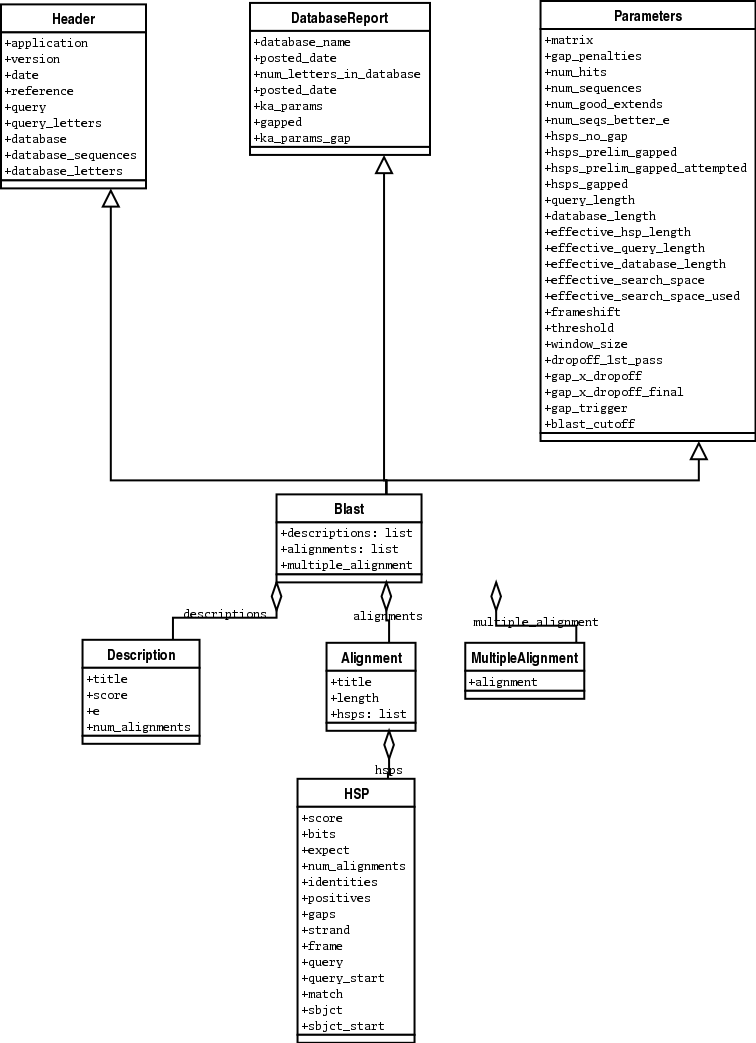
\includegraphics[width=0.8\textwidth]{images/BlastRecord.png}
\caption{Class diagram for the Blast Record class representing all of the info in a BLAST report}
\label{fig:blastrecord}
\end{figure}
\end{latexonly}

The PSIBlast record object is similar, but has support for the rounds that are used in the iteration steps of PSIBlast. The class diagram for PSIBlast is shown in Figure~\ref{fig:psiblastrecord}.

\begin{htmlonly}
\label{fig:psiblastrecord}
\imgsrc[width=650, height=750]{images/PSIBlastRecord.png}
\end{htmlonly}

\begin{latexonly}
\begin{figure}[htbp]
\centering
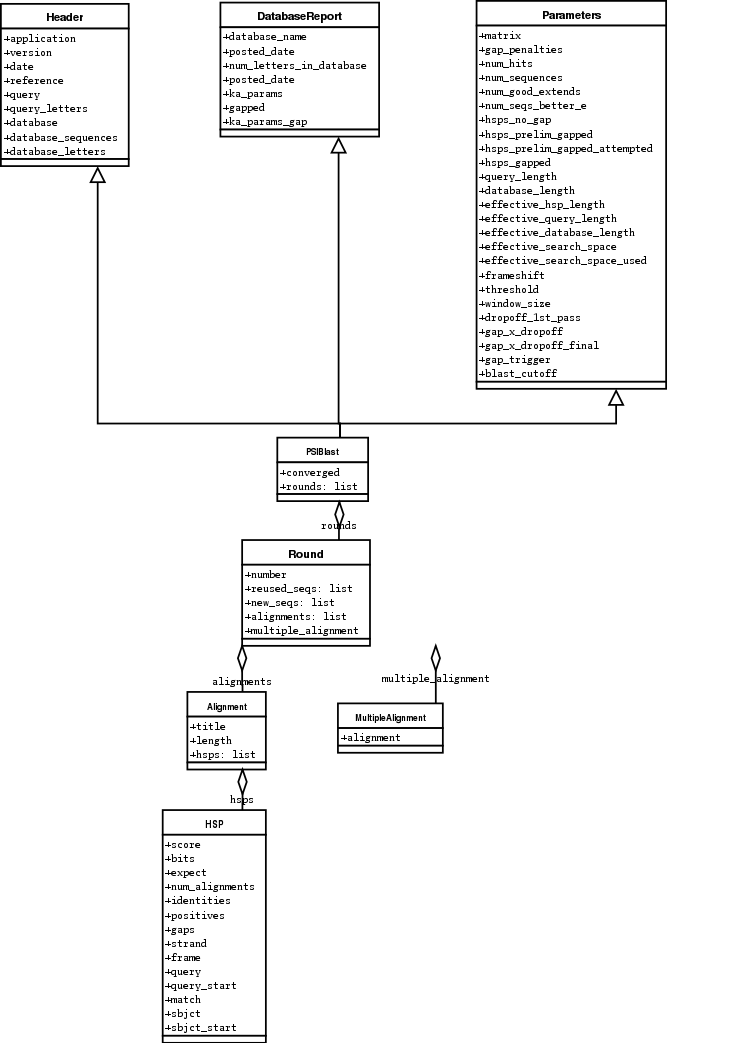
\includegraphics[width=0.8\textwidth]{images/PSIBlastRecord.png}
\caption{Class diagram for the PSIBlast Record class.}
\label{fig:psiblastrecord}
\end{figure}
\end{latexonly}

\subsection{Running BLAST locally}

If you want to make your own database to search for sequences against, then local BLAST is definitely the way you want to go. As with online BLAST, biopython provides lots of nice code to make you able to call local BLAST executables from your scripts, and have full access to the many command line options that these executables provide. You can obtain local BLAST precompiled for a number of platforms at \ahrefurl{\url{ftp://ncbi.nlm.nih.gov/blast/executables/}}, or can compile it yourself in the NCBI toolbox (\ahrefurl{\url{ftp://ncbi.nlm.nih.gov/toolbox/}}).


The code for dealing with local BLAST is found in \verb|Bio.Blast.NCBIStandalone|, specifically in the functions \verb|blastall| and \verb|blastpgp|, which correspond with the BLAST executables that their names imply.


Let's use these functions to run a \verb|blastall| against a local database and return the results. First, we want to set up the paths to everything that we'll need to do the blast. What we need to know is the path to the database (which should have been prepared using \verb|formatdb|) to search against, the path to the file we want to search, and the path to the \verb|blastall| executable.

\begin{verbatim}
import os

my_blast_db = os.path.join(os.getcwd(), 'at-est', 'a_cds-10-7.fasta')
my_blast_file = os.path.join(os.getcwd(), 'at-est', 'test_blast',
                             'sorghum_est-test.fasta')
my_blast_exe = os.path.join(os.getcwd(), 'blast', 'blastall')
\end{verbatim}

Now that we've got that all set, we are ready to run the blast and collect the results. We can do this with two lines:

\begin{verbatim}
from Bio.Blast import NCBIStandalone

blast_out, error_info = NCBIStandalone.blastall(my_blast_exe, 'blastn',
                                                my_blast_db, my_blast_file)
\end{verbatim}

Note that the biopython interfaces to local blast programs returns two values. The first is a handle to the blast output, which is ready to either be saved or passed to a parser. The second is the possible error output generated by the blast command.


The error info can be hard to deal with, because if you try to do a \verb|error_info.read()| and there was no error info returned, then the \verb|read()| call will block and not return, locking your script. In my opinion, the best way to deal with the error is only to print it out if you are not getting \verb|blast_out| results to be parsed, but otherwise to leave it alone.


If you are interested in saving your results to a file before parsing them, see the section on WWW blast above for some info on how to use the \verb|copy| module to do this.


Well, now that you've got output, we should start parsing them, so read on to learn about parsing local BLAST output.

\subsection{Parsing BLAST output from local BLAST}

Since the output generated by local BLAST is different than that generated by the web-based BLAST, we use the parsers located in \verb|Bio.Blast.NCBIStandalone| to parse and deal with the results.


As with WWW blast (see the info on this above) we need to have a handle object that we can pass to the parser. The handle must implement the \verb|readline()| method and do this properly. The common ways to get such a handle are to either use the provided \verb|blastall| or \verb|blastpgp| functions to run the local blast, or to run a local blast via the command line, and then do something like the following:

\begin{verbatim}
blast_out = open('my_file_of_blast_output', 'r')
\end{verbatim}

So, as with WWW blast, there is no need to use the biopython convenience functions if you don't want to.


Well, now that we've got a handle (which we'll call \verb|blast_out|), we are ready to parse it. This can be done with the following code:

\begin{verbatim}
from Bio.Blast import NCBIStandalone

b_parser = NCBIStandalone.BlastParser()
b_record = b_parser.parse(blast_out)
\end{verbatim} 

This will parse the BLAST report into a Blast Record class (either a Blast or a PSIBlast record, depending on what you are parsing) so that you can extract the information from it. In our case, let's just use print out a quick summary of all of the alignments greater than some threshold value.

\begin{verbatim}
E_VALUE_THRESH = 0.04
for alignment in b_record.alignments:
    for hsp in alignment.hsps:
        if hsp.expect < E_VALUE_THRESH:
            print '****Alignment****'
            print 'sequence:', alignment.title
            print 'length:', alignment.length
            print 'e value:', hsp.expect
            print hsp.query[0:75] + '...'
            print hsp.match[0:75] + '...'
            print hsp.sbjct[0:75] + '...'
\end{verbatim}

If you also read the section on parsing BLAST from the WWW version, you'll notice that the above code is identical to what is found in that section. Once you parse something into a record class you can deal with it independent of the format of the original BLAST info you were parsing. Pretty snazzy!


Sure, parsing one record is great, but I've got a BLAST file with tons of records -- how can I parse them all? Well, fear not, the answer lies in the very next section.

\subsection{Parsing a file full of BLAST runs}

Of course, local blast is cool because you can run a whole bunch of sequences against a database and get back a nice report on all of it. So, biopython definitely has facilities to make it easy to parse humongous files without memory problems. 


We can do this using the blast iterator. To set up an iterator, we first set up a parser, to parse our blast reports in Blast Record objects:

\begin{verbatim}
from Bio.Blast import NCBIStandalone

b_parser = NCBIStandalone.BlastParser()
\end{verbatim}

Then we will assume we have a handle to a bunch of blast records, which we'll call \verb|blast_out|. Getting a handle is described in full detail above in the blast parsing sections. 


Now that we've got a parser and a handle, we are ready to set up the iterator with the following command:

\begin{verbatim}
b_iterator = NCBIStandalone.Iterator(blast_out, b_parser)
\end{verbatim}

The second option, the parser, is optional. If we don't supply a parser, then the iterator will just return the raw BLAST reports one at a time.


Now that we've got an iterator, we start retrieving blast records (generated by our parser) using \verb|next()|:

\begin{verbatim}
b_record = b_iterator.next()
\end{verbatim}

Each call to next will return a new record that we can deal with. Now we can iterate through this records and generate our old favorite, a nice little blast report:

\begin{verbatim}
while 1:
    b_record = b_iterator.next()

    if b_record is None:
        break

    E_VALUE_THRESH = 0.04
    for alignment in b_record.alignments:
        for hsp in alignment.hsps:
            if hsp.expect < E_VALUE_THRESH:
                print '****Alignment****'
                print 'sequence:', alignment.title
                print 'length:', alignment.length
                print 'e value:', hsp.expect

                if len(hsp.query) > 75:
                    dots = '...'
                else:
                    dots = ''
                
                print hsp.query[0:75] + dots
                print hsp.match[0:75] + dots
                print hsp.sbjct[0:75] + dots
\end{verbatim}

Notice that \verb|b_iterator.next()| will return \verb|None| when it runs out of records to parse, so it is easy to iterate through the entire file with a while loop that checks for the existence of a record.


The iterator allows you to deal with huge blast records without any memory problems, since things are read in one at a time. I have parsed tremendously huge files without any problems using this.

\subsection{Finding a bad record somewhere in a huge file}

One really ugly problem that happens to me is that I'll be parsing a huge blast file for a while, and the parser will bomb out with a SyntaxError. This is a serious problem, since you can't tell if the SyntaxError is due to a parser problem, or a problem with the BLAST. To make it even worse, you have no idea where the parse failed, so you can't just ignore the error, since this could be ignoring an important data point.


We used to have to make a little script to get around this problem, but the \verb|Bio.Blast| module now includes a \verb|BlastErrorParser| which really helps make this easier. The \verb|BlastErrorParser| works very similar to the regular \verb|BlastParser|, but it adds an extra layer of work by catching SyntaxErrors that are generated by the parser, and attempting to diagnose the errors.


Let's take a look at using this parser -- first we define the file we are going to parse and the file to write the problem reports to:

\begin{verbatim}
import os
 
b_file = os.path.join(os.getcwd(), 'blast_out', 'big_blast.out')
error_file = os.path.join(os.getcwd(), 'blast_out', 'big_blast.problems')
\end{verbatim}

Now we want to get a \verb|BlastErrorParser|:

\begin{verbatim}
from Bio.Blast import NCBIStandalone

error_handle = open(error_file, 'w')

b_error_parser = NCBIStandalone.BlastErrorParser(error_handle)
\end{verbatim}

Notice that the parser take an optional argument of a handle. If a handle is passed, then the parser will write any blast records which generate a SyntaxError to this handle. Otherwise, these records will not be recorded.


Now we can use the \verb|BlastErrorParser| just like a regular blast parser. Specifically, we might want to make an iterator that goes through our blast records one at a time and parses them with the error parser:

\begin{verbatim}
blast_out = open(b_file)
iterator = NCBIStandalone.Iterator(blast_out, b_error_parser)
\end{verbatim}

Just like before, we can read these records one a time with, but now we can catch and deal with errors that are due to problems with Blast (and not with the parser itself):

\begin{verbatim}
try:
    next_record = iterator.next()
except NCBIStandalone.LowQualityBlastError, info:
    print "LowQualityBlastError detected in id %s" % info[1]
\end{verbatim}

Right now the \verb|BlastErrorParser| can generate the following errors:

\begin{itemize}
  \item \verb|SyntaxError| -- This is the same error generated by the regular BlastParser, and is due to the parser not being able to parse a specific file. This is normally either due to a bug in the parser, or some kind of discrepancy between the version of BLAST you are using and the versions the parser is able to handle.

  \item \verb|LowQualityBlastError| -- When BLASTing a sequence that is of really bad quality (for example, a short sequence that is basically a stretch of one nucleotide), it seems that Blast ends up masking out the entire sequence and ending up with nothing to parse. In this case it will produce a truncated report that causes the parser to generate a SyntaxError. \verb|LowQualityBlastError| is reported in these cases. This error returns an info item with the following information:
  \begin{itemize}
    \item \verb|item[0]| -- The error message
    \item \verb|item[1]| -- The id of the input record that caused the error. This is really useful if you want to record all of the records that are causing problems.
  \end{itemize}
\end{itemize}

As mentioned, with each error generated, the BlastErrorParser will write the offending record to the specified \verb|error_handle|. You can then go ahead and look and these and deal with them as you see fit. Either you will be able to debug the parser with a single blast report, or will find out problems in your blast runs. Either way, it will definitely be a useful experience!


Hopefully the \verb|BlastErrorParser| will make it much easier to debug and deal with large Blast files.

\subsection{Dealing with PSIBlast}

We should write some stuff to make it easier to deal directly with PSIBlast from scripts (i.~e.~output the align file in the proper format from an alignment). I need to look at PSIBlast more and come up with some good ways of going this...

\section{SWISS-PROT}
\label{sec:swiss_prot}

\subsection{Retrieving a SWISS-PROT record}

SwissProt (\ahrefurl{\url{http://www.expasy.org/sprot/sprot-top.html}}) is a hand-curated database of protein sequences. Let's look at how we connect with it from a script and parse SwissProt formatted results. 


First, we need to retrieve some results to parse. Let's say we are looking at chalcone synthases for Orchids (see section~\ref{sec:orchids} for some justification for looking for interesting things about orchids). Chalcone synthase is involved in flavanoid biosynthesis in plants, and flavanoids make lots of cool things like pigment colors and UV protectants. 


If you do a search on SwissProt, you can find three orchid proteins for Chalcone Synthase, id numbers O23729, O23730, O23731. Now, let's write a script which grabs these, and parses out some interesting information.


First, we grab the records, using the \verb|get_sprot_raw()| function of \verb|Bio.WWW.ExPASy|. This function is very nice since you can feed it an id and get back a raw text record (no html to mess with!). As we get the three records we are interested in, we'll just put them together into one big string, which we'll then use for parsing. The following code accomplishes what I just wrote:

\begin{verbatim}
from Bio.WWW import ExPASy

ids = ['O23729', 'O23730', 'O23731']

all_results = ''
for eid in ids:
    results = ExPASy.get_sprot_raw(eid)
    all_results = all_results + results.read()
\end{verbatim}

Now that we've got the results, we are ready to parse them into interesting information. As with most parsers, we set up an iterator and parser. The parser we use here parses the SwissProt files into a Record object where the interesting features are attributes:

\begin{verbatim}
from Bio.SwissProt import SProt
from Bio import File

s_parser = SProt.RecordParser()
s_iterator = SProt.Iterator(File.StringHandle(all_results), s_parser)
\end{verbatim}

Note that we convert \verb|all_results|, which is a string, into a handle before passing it. The iterator requires a handle to be passed so that it can read in everything one line at a time. The \verb|Bio.File| module has a nice StringHandle, which conveniently will convert a string into a handle. Very nice! Now we are ready to start extracting information.


To get out the information, we'll go through everything record by record using the iterator. For each record, we'll just print out some summary information:

\begin{verbatim}
while 1:
    cur_record = s_iterator.next()

    if cur_record is None:
        break

    print "description:", cur_record.description
    for ref in cur_record.references:
        print "authors:", ref.authors
        print "title:", ref.title

    print "classification:", cur_record.organism_classification
    print
\end{verbatim}

This prints out a summary like the following:

\begin{verbatim}
description: CHALCONE SYNTHASE 8 (EC 2.3.1.74) (NARINGENIN-CHALCONE SYNTHASE 8)
authors: Liew C.F., Lim S.H., Loh C.S., Goh C.J.;
title: "Molecular cloning and sequence analysis of chalcone synthase cDNAs of
Bromheadia finlaysoniana.";
classification: ['Eukaryota', 'Viridiplantae', 'Embryophyta', 'Tracheophyta', 
'Spermatophyta', 'Magnoliophyta', 'Liliopsida', 'Asparagales', 'Orchidaceae', 
'Bromheadia']
\end{verbatim}

Since Python 2.2, we can simplify the loop:

\begin{verbatim}
for cur_record in s_iterator:
    print "description:", cur_record.description
    for ref in cur_record.references:
        print "authors:", ref.authors
        print "title:", ref.title

    print "classification:", cur_record.organism_classification
    print
\end{verbatim}


It is equally easy to extract any kind of information you'd like from SwissProt records.


Now, you may remark that I knew the records' accession numbers
beforehand. Indeed, \verb|get_sprot_raw()| needs either the entry name
or an accession number. When you don't have them handy, you can use
one of the \verb|sprot_search_de()| or \verb|sprot_search_ful()|
functions.

\verb|sprot_search_de()| searches in the ID, DE, GN, OS and OG lines;
\verb|sprot_search_ful()| searches in (nearly) all the fields. They
are detailed on
\ahrefurl{\url{http://www.expasy.org/cgi-bin/sprot-search-de}} and
\ahrefurl{\url{http://www.expasy.org/cgi-bin/sprot-search-ful}}
respectively. Note that thet don't search in TrEMBL by default
(argument \verb|trembl|). Note also that they return html pages;
however, accession numbers are quite easily extractable:

\begin{verbatim}
from Bio.WWW import ExPASy
import re

handle = ExPASy.sprot_search_de("Orchid Chalcone Synthase")
# or:
# handle = ExPASy.sprot_search_ful("Orchid and {Chalcone Synthase}")
html_results = handle.read()
if "Number of sequences found" in html_results:
    ids = re.findall(r'HREF="/cgi-bin/niceprot\.pl\?(\w+)"', html_results)
else:
    ids = re.findall(r'href="/cgi-bin/get-sprot-raw\.pl\?(\w+)"', html_results)
\end{verbatim}

\section{PubMed}
\label{sec:pub_med}

\subsection{Sending a query to PubMed}

If you are in the Medical field or interested in human issues (and many times even if you are not!), PubMed (\ahrefurl{\url{http://www.ncbi.nlm.nih.gov/PubMed/}}) is an excellent source of all kinds of goodies. So like other things, we'd like to be able to grab information from it and use it in python scripts.


Querying PubMed using Biopython is extremely painless. To get all of the article ids for articles having to do with orchids, we only need the following three lines of code:

\begin{verbatim}
from Bio import PubMed

search_term = 'orchid'
orchid_ids = PubMed.search_for(search_term)
\end{verbatim}

This returns a python list containing all of the orchid ids

\begin{verbatim}
['11070358', '11064040', '11028023', '10947239', '10938351', '10936520', 
'10905611', '10899814', '10856762', '10854740', '10758893', '10716342', 
...
\end{verbatim}

With this list of ids we are ready to start retrieving the records, so follow on ahead to the next section.

\subsection{Retrieving a PubMed record}

The previous section described how to get a bunch of article ids. Now that we've got them, we obviously want to get the corresponding Medline records and extract the information from them. 


The interface for retrieving records from PubMed should be very intuitive to python programmers -- it models a python dictionary. To set up this interface, we need to set up a parser that will parse the results that we retrieve. The following lines of code get everything set up:

\begin{verbatim}
from Bio import PubMed
from Bio import Medline

rec_parser = Medline.RecordParser()
medline_dict = PubMed.Dictionary(parser = rec_parser)
\end{verbatim}

What we've done is create a dictionary like object \verb|medline_dict|. To get an article we access it like \verb|medline_dict[id_to_get]|. What this does is connect with PubMed, get the article you ask for, parse it into a record object, and return it. Very cool! 


Now let's look at how to use this nice dictionary to print out some information about some ids. We just need to loop through our ids (\verb|orchid_ids| from the previous section) and print out the information we are interested in:

\begin{verbatim}
for oid in orchid_ids[0:5]:
    cur_record = medline_dict[oid]
    print 'title:', string.rstrip(cur_record.title)
    print 'authors:', cur_record.authors
    print 'source:', string.strip(cur_record.source)
    print
\end{verbatim}

The output for this looks like:

\begin{verbatim}
title: Sex pheromone mimicry in the early spider orchid (ophrys sphegodes):
patterns of hydrocarbons as the key mechanism for pollination by sexual
deception [In Process Citation]
authors: ['Schiestl FP', 'Ayasse M', 'Paulus HF', 'Lofstedt C', 'Hansson BS', 
'Ibarra F', 'Francke W']
source: J Comp Physiol [A] 2000 Jun;186(6):567-74
\end{verbatim}

Especially interesting to note is the list of authors, which is returned as a standard python list. This makes it easy to manipulate and search using standard python tools. For instance, we could loop through a whole bunch of entries searching for a particular author with code like the following:

\begin{verbatim}
search_author = 'Waits T'

for our_id in our_id_list:
    cur_record = medline_dict[our_id]
    
    if search_author in cur_record.authors:
        print "Author %s found: %s" % (search_author,
                                       string.strip(cur_record.source))
\end{verbatim} 

The PubMed and Medline interfaces are very mature and nice to work with -- hopefully this section gave you an idea of the power of the interfaces and how they can be used.

\section{GenBank}

The GenBank record format is a very popular method of holding information about sequences, sequence features, and other associated sequence information. The format is a good way to get information from the NCBI databases at \ahrefurl{\url{http://www.ncbi.nlm.nih.gov/}}. 

\subsection{Retrieving GenBank entries from NCBI}

One very nice feature of the GenBank libraries is the ability to automate retrieval of entries from GenBank. This is very convenient for creating scripts that automate a lot of your daily work. In this example we'll show how to query the NCBI databases, and to retrieve the records from the query.


First, we want to make a query and find out the ids of the records to retrieve. Here we'll do a quick search for \emph{Opuntia}, my favorite organism (since I work on it). We can do quick search and get back the GIs (GenBank identifiers) for all of the corresponding records:

\begin{verbatim}
from Bio import GenBank

gi_list = GenBank.search_for("Opuntia AND rpl16")
\end{verbatim}

\verb|gi_list| will be a list of all of the GenBank identifiers that match our query:

\begin{verbatim}
['6273291', '6273290', '6273289', '6273287', '6273286', '6273285', '6273284']
\end{verbatim}

Now that we've got the GIs, we can use these to access the NCBI database through a dictionary interface. For instance, to retrieve the information for the first GI, we'll first have to create a dictionary that accesses NCBI:

\begin{verbatim}
ncbi_dict = GenBank.NCBIDictionary('nucleotide', 'genbank')
\end{verbatim}

Now that we've got this, we do the retrieval:

\begin{verbatim}
gb_record = ncbi_dict[gi_list[0]]
\end{verbatim}

In this case, \verb|gb_record| will be GenBank formatted record:

\begin{verbatim}
LOCUS       AF191665      902 bp    DNA             PLN       07-NOV-1999
DEFINITION  Opuntia marenae rpl16 gene; chloroplast gene for chloroplast
            product, partial intron sequence.
ACCESSION   AF191665
VERSION     AF191665.1  GI:6273291
...
\end{verbatim}

In this case, we are just getting the raw records. We can also pass these records directly into a parser and return the parsed record. For instance, if we wanted to get back SeqRecord objects with the GenBank file parsed into SeqFeature objects we would need to create the dictionary with the GenBank FeatureParser:

\begin{verbatim}
record_parser = GenBank.FeatureParser()
ncbi_dict = GenBank.NCBIDictionary('nucleotide', 'genbank',
                                   parser = record_parser)
\end{verbatim}

Now retrieving a record will give you a SeqRecord object instead of the raw record:

\begin{verbatim}
>>> gb_seqrecord = ncbi_dict[gi_list[0]]
>>> print gb_seqrecord
<Bio.SeqRecord.SeqRecord instance at 0x102f9404>
\end{verbatim}

For more information of formats you can parse GenBank records into, please see section~\ref{sec:gb-parsing}.


Using these automated query retrieval functionality is a big plus over doing things by hand. Additionally, the retrieval has nice built in features like a time-delay, which will prevent NCBI from getting mad at you and blocking your access.

\subsection{Parsing GenBank records}
\label{sec:gb-parsing}

While GenBank files are nice and have lots of information, at the same time you probably only want to extract a small amount of that information at a time. The key to doing this is parsing out the information. Biopython provides GenBank parsers which help you accomplish this task. Right now the GenBank module provides the following parsers:

\begin{enumerate}
  \item RecordParser -- This parses the raw record into a GenBank specific Record object. This object models the information in a raw record very closely, so this is good to use if you are just interested in GenBank records themselves.

  \item FeatureParser -- This parses the raw record in a SeqRecord object with all of the feature table information represented in SeqFeatures (see section~\ref{sec:advanced-seq} for more info on these objects). This is best to use if you are interested in getting things in a more standard format.
\end{enumerate}

Either way you chose to go, the most common usage of these will be creating an iterator and parsing through a file on GenBank records. Doing this is very similar to how things are done in other formats, as the following code demonstrates:

\begin{verbatim}
from Bio import GenBank

gb_file = "my_file.gb"
gb_handle = open(gb_file, 'r')

feature_parser = GenBank.FeatureParser()

gb_iterator = GenBank.Iterator(gb_handle, feature_parser)

while 1:
   cur_record = gb_iterator.next()

   if cur_record is None:
       break

   # now do something with the record
   print cur_record.seq
\end{verbatim}

This just iterates over a GenBank file, parsing it into SeqRecord and SeqFeature objects, and prints out the Seq objects representing the sequences in the record.


As with other formats, you have lots of tools for dealing with GenBank records. This should make it possible to do whatever you need to with GenBank.

\subsection{Making your very own GenBank database}

One very cool thing that you can do is set up your own personal GenBank database and access it like a dictionary (this can be extra cool because you can also allow access to these local databases over a network using BioCorba -- see the BioCorba documentation for more information).


Making a local database first involves creating an index file, which will allow quick access to any record in the file. To do this, we use the index file function:

\begin{verbatim}
>>> from Bio import GenBank
>>> dict_file = 'cor6_6.gb'
>>> index_file = 'cor6_6.idx'
>>> GenBank.index_file(dict_file, index_file)
\end{verbatim}

This will create the file \verb|my_index_file.idx|. Now, we can use this index to create a dictionary object that allows individual access to every record. Like the Iterator and NCBIDictionary interfaces, we can either get back raw records, or we can pass the dictionary a parser that will parse the records before returning them. In this case, we pass a \verb|FeatureParser| so that when we get a record, then we retrieve a SeqRecord object. 


Setting up the dictionary is as easy as one line:

\begin{verbatim}
>>> gb_dict = GenBank.Dictionary(index_file, GenBank.FeatureParser())
\end{verbatim}

Now we can deal with this like a dictionary. For instance:

\begin{verbatim}
>>> len(gb_dict)
7
>>> gb_dict.keys()
['L31939', 'AJ237582', 'X62281', 'AF297471', 'M81224', 'X55053']
\end{verbatim}

Finally, we retrieve objects using subscripting:

\begin{verbatim}
>>> gb_dict['AJ237582']
<Bio.SeqRecord.SeqRecord instance at 0x102fdd8c>
\end{verbatim}

\section{Dealing with alignments}

It is often very useful to be able to align particular sequences. I do this quite often to get a quick and dirty idea of relationships between sequences. Consequently, it is very nice to be able to quickly write up a python script that does an alignment and gives you back objects that are easy to work with. The alignment related code in Biopython is meant to allow python-level access to alignment programs so that you can run alignments quickly from within scripts.

\subsection{Clustalw}
\label{sec:align_clustal}

Clustalx (\ahrefurl{\url{http://www-igbmc.u-strasbg.fr/BioInfo/ClustalX/Top.html}}) is a very nice program for doing multiple alignments. Biopython offers access to alignments in clustal format (these normally have a \verb|*.aln| extension) that are produced by Clustalx. It also offers access to clustalw, which the is command line version of clustalx.


The first step in interacting with clustalw is to set up a command line you want to pass to the program. Clustalw has a ton of command line options, and if you set a lot of parameters, you can end up typing in a huge ol' command line quite a bit. This command line class models the command line by making all of the options be attributes of the class that can be set. A few convenience functions also exist to set certain parameters, so that some error checking on the parameters can be done.


To create a command line object to do a clustalw multiple alignment we do the following:

\begin{verbatim}
import os
from Bio.Clustalw import MultipleAlignCL

cline = MultipleAlignCL(os.path.join(os.curdir, 'opuntia.fasta'))
cline.set_output('test.aln')
\end{verbatim}

First we import the \verb|MultipleAlignCL| object, which models running a multiple alignment from clustalw. We then initialize the command line, with a single argument of the fasta file that we are going to be using for the alignment. The initialization function also takes an optional second argument which specifies the location of the \verb|clustalw| executable. By default, the commandline will just be invoked with 'clustalw,' assuming that you've got it somewhere on your \verb|PATH|.


The second argument sets the output to go to the file \verb|test.aln|. The \verb|MultipleAlignCL| object also has numerous other parameters to specify things like output format, gap costs, etc. 


We can look at the command line we have generated by invoking the \verb|__str__| member attribute of the \verb|MultipleAlignCL| class. This is done by calling \verb|str(cline)| or simple by printing out the command line with \verb|print cline|. In this case, doing this would give the following output:

\begin{verbatim}
clustalw ./opuntia.fasta -OUTFILE=test.aln
\end{verbatim}

Now that we've set up a simple command line, we now want to run the commandline and collect the results so we can deal with them. This can be done using the \verb|do_alignment| function of \verb|Clustalw| as follows:

\begin{verbatim}
from Bio import Clustalw

alignment = Clustalw.do_alignment(cline)
\end{verbatim}

What happens when you run this if that Biopython executes your command line and runs clustalw with the given parameters. It then grabs the output, and if it is in a format that Biopython can parse (currently only clustal format), then it will parse the results and return them as an alignment object of the appropriate type. So in this case since we are getting results in the default clustal format, the returned \verb|alignment| object will be a \verb|ClustalAlignment| type.


Once we've got this alignment, we can do some interesting things with it such as get \verb|seq_record| objects for all of the sequences involved in the alignment:

\begin{verbatim}
all_records = alignment.get_all_seqs()

print 'description:', all_records[0].description
print 'sequence:', all_records[0].seq
\end{verbatim}

This prints out the description and sequence object for the first sequence in the alignment:

\begin{verbatim}
description: gi|6273285|gb|AF191659.1|AF191
sequence: Seq('TATACATTAAAGAAGGGGGATGCGGATAAATGGAAAGGCGAAAGAAAGAAAAAAATGAAT 
...', IUPACAmbiguousDNA())
\end{verbatim}

You can also calculate the maximum length of the alignment with:

\begin{verbatim}
length = alignment.get_alignment_length()
\end{verbatim}

Finally, to write out the alignment object in the original format, we just need to access the \verb|__str__| function. So doing a \verb|print alignment| gives:

\begin{verbatim}
CLUSTAL X (1.81) multiple sequence alignment


gi|6273285|gb|AF191659.1|AF191      TATACATTAAAGAAGGGGGATGCGGATAAATGGAAAGGCGAAAGAAAGAA
gi|6273284|gb|AF191658.1|AF191      TATACATTAAAGAAGGGGGATGCGGATAAATGGAAAGGCGAAAGAAAGAA
...
\end{verbatim}

This makes it easy to write your alignment back into a file with all of the original info intact.


If you want to do more interesting things with an alignment, the best thing to do is to pass the alignment to an alignment information generating object, such as the SummaryInfo object, described in section~\ref{sec:summary_info}.

\subsection{Calculating summary information}
\label{sec:summary_info}

Once you have an alignment, you are very likely going to want to find out information about it. Instead of trying to have all of the functions that can generate information about an alignment in the alignment object itself, we've tried to separate out the functionality into separate classes, which act on the alignment. 


Getting ready to calculate summary information about an object is quick to do. Let's say we've got an alignment object called \verb|alignment|. All we need to do to get an object that will calculate summary information is:

\begin{verbatim}
from Bio.Align import AlignInfo
summary_align = AlignInfo.SummaryInfo(alignment)
\end{verbatim}

The \verb|summary_align| object is very useful, and will do the following neat things for you:

\begin{enumerate}
  \item Calculate a quick consensus sequence -- see section~\ref{sec:consensus}
  \item Get a position specific score matrix for the alignment -- see section~\ref{sec:pssm}
  \item Calculate the information content for the alignment -- see section~\ref{sec:getting_info_content}
  \item Generate information on substitutions in the alignment -- section~\ref{sec:sub_matrix} details using this to generate a substitution matrix.
\end{enumerate}

\subsection{Calculating a quick consensus sequence}
\label{sec:consensus}

The \verb|SummaryInfo| object, described in section~\ref{sec:summary_info}, provides functionality to calculate a quick consensus of an alignment. Assuming we've got a \verb|SummaryInfo| object called \verb|summary_align| we can calculate a consensus by doing:

\begin{verbatim}
consensus = summary_align.dumb_consensus()
\end{verbatim}

As the name suggests, this is a really simple consensus calculator, and will just add up all of the residues at each point in the consensus, and if the most common value is higher than some threshold value (the default is .3) will add the common residue to the consensus. If it doesn't reach the threshold, it adds an ambiguity character to the consensus. The returned consensus object is Seq object whose alphabet is inferred from the alphabets of the sequences making up the consensus. So doing a \verb|print consensus| would give:

\begin{verbatim}
consensus Seq('TATACATNAAAGNAGGGGGATGCGGATAAATGGAAAGGCGAAAGAAAGAAAAAAATGAAT 
...', IUPACAmbiguousDNA())
\end{verbatim} 

You can adjust how \verb|dumb_consensus| works by passing optional parameters:

\begin{description}
\item[the threshold] This is the threshold specifying how common a particular residue has to be at a position before it is added. The default is .7.

\item[the ambiguous character] This is the ambiguity character to use. The default is 'N'.

\item[the consensus alphabet] This is the alphabet to use for the consensus sequence. If an alphabet is not specified than we will try to guess the alphabet based on the alphabets of the sequences in the alignment.
\end{description}

\subsection{Position Specific Score Matrices}
\label{sec:pssm}

Position specific score matrices (PSSMs) summarize the alignment information in a different way than a consensus, and may be useful for different tasks. Basically, a PSSM is a count matrix. For each column in the alignment, the number of each alphabet letters is counted and totaled. The totals are displayed relative to some representative sequence along the left axis. This sequence may be the consesus sequence, but can also be any sequence in the alignment. For instance for the alignment:

\begin{verbatim}
GTATC
AT--C
CTGTC
\end{verbatim}

the PSSM for this alignment is:

\begin{verbatim}
      G A T C
    G 1 1 0 1
    T 0 0 3 0
    A 1 1 0 0
    T 0 0 2 0
    C 0 0 0 3
\end{verbatim}

Let's assume we've got an alignment object called \verb|c_align|. To get a PSSM with the consensus sequence along the side we first get a summary object and calculate the consensus sequence:

\begin{verbatim}
summary_align = AlignInfo.SummaryInfo(c_align)
consensus = summary_align.dumb_consensus()
\end{verbatim}

Now, we want to make the PSSM, but ignore any \verb|N| ambiguity residues when calculating this:

\begin{verbatim}
my_pssm = summary_align.pos_specific_score_matrix(consensus,
                                                  chars_to_ignore = ['N'])
\end{verbatim}

Two notes should be made about this:

\begin{enumerate}
  \item To maintain strictness with the alphabets, you can only include characters along the top of the PSSM that are in the alphabet of the alignment object. Gaps are not included along the top axis of the PSSM.

  \item The sequence passed to be displayed along the left side of the axis does not need to be the consensus. For instance, if you wanted to display the second sequence in  the alignment along this axis, you would need to do:

\begin{verbatim}
second_seq = alignment.get_seq_by_num(1)
my_pssm = summary_align.pos_specific_score_matrix(second_seq
                                                  chars_to_ignore = ['N'])
\end{verbatim}

\end{enumerate}

The command above returns a \verb|PSSM| object. To print out the PSSM as we showed above, we simply need to do a \verb|print my_pssm|, which gives:

\begin{verbatim}
    A   C   G   T
T  0.0 0.0 0.0 7.0
A  7.0 0.0 0.0 0.0
T  0.0 0.0 0.0 7.0
A  7.0 0.0 0.0 0.0
C  0.0 7.0 0.0 0.0
A  7.0 0.0 0.0 0.0
T  0.0 0.0 0.0 7.0
T  1.0 0.0 0.0 6.0
...
\end{verbatim}

You can access any element of the PSSM by subscripting like \verb|your_pssm[sequence_number][residue_count_name]|. For instance, to get the counts for the 'A' residue in the second element of the above PSSM you would do:

\begin{verbatim}
>>> print my_pssm[1]['A']
7.0
\end{verbatim}

The structure of the PSSM class hopefully makes it easy both to access elements and to pretty print the matrix.

\subsection{Information Content}
\label{sec:getting_info_content}

A potentially useful measure of evolutionary conservation is the information ceontent of a sequence.


A useful introduction to information theory targetted towards molecular biologists can be found at \ahrefurl{\url{http://www.lecb.ncifcrf.gov/~toms/paper/primer/}}. For our purposes, we will be looking at the information content of a consesus sequence, or a portion of a consensus sequence. We calculate information content at a particular column in a multiple sequence alignment using the following formula:

\begin{displaymath}
IC_{j} = \sum_{i=1}^{N_{a}} P_{ij} * log(\frac{P_{ij}}{Q_{i}}) 
\end{displaymath}

where:

\begin{itemize}
  \item $IC_{j}$ -- The information content for the jth column in an alignment.
  \item $N_{a}$ -- The number of letters in the alphabet.
  \item $P_{ij}$ -- The frequency of a particular letter in the column (i.~e.~if G occured 3 out of 6 times in an aligment column, this would be 0.5)
  \item $Q_{i}$ --  The expected frequency of a letter. This is an
  optional argument, usage of which is left at the user's
  discretion. By default, it is automatically assigned to 0.05 for a
  protein alphabet, and 0.25 for a nucleic acid alphabet. This is for
  geting the information content without any assumption of prior
  distribtions. When assuming priors, or when using a non-standard
  alphabet, user should supply the values for $Q_{i}$. 
\end{itemize}

Well, now that we have an idea what information content is being calculated in Biopython, let's look at how to get it for a particular region of the alignment.


First, we need to use our alignment to get a alignment summary object, which we'll assume is called \verb|summary_align| (see section~\ref{sec:summary_info}) for instructions on how to get this. Once we've got this object, calculating the information content for a region is as easy as:

\begin{verbatim}
info_content = summary_align.information_content(5, 30, 
                                                 chars_to_ignore = ['N'])
\end{verbatim}

Wow, that was much easier then the formula above made it look! The variable \verb|info_content| now contains a float value specifying the information content over the specified region (from 5 to 30 of the alignment). We specifically ignore the ambiguity residue 'N' when calculating the information content, since this value is not included in our alphabet (so we shouldn't be interested in looking at it!).


As mentioned above, we can also calculate relative information content by supplying the expected frequencies:

\begin{verbatim}
expect_freq = {
    'A' : .3,
    'G' : .2,
    'T' : .3,
    'C' : .2}
\end{verbatim}

The expected should not be passed as a raw dictionary, but instead by passed as a \verb|SubsMat.FreqTable| object (see section~\ref{sec:freq_table} for more information about FreqTables). The FreqTable object provides a standard for associating the dictionary with an Alphabet, similar to how the Biopython Seq class works. 


To create a FreqTable object, from the frequency dictionary you just need to do:

\begin{verbatim}
from Bio.Alphabet import IUPAC
from Bio.SubsMat import FreqTable

e_freq_table = FreqTable.FreqTable(expect_freq, FreqTable.FREQ,
                                   IUPAC.unambigous_dna)
\end{verbatim}

Now that we've got that, calculating the relative information content for our region of the alignment is as simple as:


\begin{verbatim}
info_content = summary_align.information_content(5, 30,
                                                 e_freq_table = e_freq_table,
                                                 chars_to_ignore = ['N'])
\end{verbatim}

Now, \verb|info_content| will contain the relative information content over the region in relation to the expected frequencies.


The value return is calculated using base 2 as the logarithm base in the formula above. You can modify this by passing the parameter \verb|log_base| as the base you want:

\begin{verbatim}
info_content = summary_align.information_content(5, 30, log_base = 10
                                                 chars_to_ignore = ['N'])
\end{verbatim}

Well, now you are ready to calculate information content. If you want to try applying this to some real life problems, it would probably be best to dig into the literature on information content to get an idea of how it is used. Hopefully your digging won't reveal any mistakes made in coding this function!

\subsection{Translating between Alignment formats}
\label{sec:align_translate}

One thing that you always end up having to do is convert between different formats. Biopython does this using a FormatConverter class for alignment objects. First, let's say we have just parsed an alignment from clustal format into a \verb|ClustalAlignment| object:

\begin{verbatim}
import os
from Bio import Clustalw

alignment = Clustalw.parse_file(os.path.join(os.curdir, 'test.aln'))
\end{verbatim}

Now, let's convert this alignment into FASTA format. First, we create a converter object:

\begin{verbatim}
from Bio.Align.FormatConvert import FormatConverter

converter = FormatConverter(alignment)
\end{verbatim}

We pass the converter the alignment that we want to convert. Now, to get this in FASTA alignment format, we simply do the following:

\begin{verbatim}
fasta_align = converter.to_fasta()
\end{verbatim}

Looking at the newly created \verb|fasta_align| object using \verb|print fasta_align| gives:

\begin{verbatim}
>gi|6273285|gb|AF191659.1|AF191
TATACATTAAAGAAGGGGGATGCGGATAAATGGAAAGGCGAAAGAAAGAATATATA----
------ATATATTTCAAATTTCCTTATATACCCAAATATAAAAATATCTAATAAATTAGA
...
\end{verbatim}

The conversion process will, of course, lose information specific to a particular alignment format. Howerver, most of the basic information about the alignment will be retained.


As more formats are added the converter will be beefed up to read and write all of these different formats.

\section{Substitution Matrices}
\label{sec:sub_matrix}

Substitution matrices are an extremely important part of everyday bioinformatics work. They provide the scoring terms for classifying how likely two different residues are to substitute for each other. This is essential in doing sequence comparisons. The book ``Biological Sequence Analysis'' by Durbin et al. provides a really nice introduction to Substitution Matrices and their uses. Some famous substitution matrices are the PAM and BLOSUM series of matrices.


Biopython provides a ton of common substitution matrices, and also provides functionality for creating your own substitution matrices.

\subsection{Using common substitution matrices}

\subsection{Creating your own substitution matrix from an alignment}
\label{sec:subs_mat_ex}

A very cool thing that you can do easily with the substitution matrix
classes is to create your own substitution matrix from an
alignment. In practice, this is normally done with protein
alignments. In this example, we'll first get a biopython alignment
object and then get a summary object to calculate info about the
alignment:


\begin{verbatim}
from Bio import Clustalw
from Bio.Alphabet import IUPAC
from Bio.Align import AlignInfo

# get an alignment object from a Clustalw alignment output
c_align = Clustalw.parse_file('protein.aln', IUPAC.protein)
summary_align = AlignInfo.SummaryInfo(c_align)
\end{verbatim}

Sections~\ref{sec:align_clustal} and~\ref{sec:summary_info} contain
more information on doing this.


Now that we've got our \verb|summary_align| object, we want to use it
to find out the number of times different residues substitute for each
other. To make the example more readable, we'll focus on only amino
acids with polar charged side chains. Luckily, this can be done easily 
when generating a replacement dictionary, by passing in all of the
characters that should be ignored. Thus we'll create a dictionary of
replacements for only charged polar amino acids using:

\begin{verbatim}
replace_info = summary_align.replacement_dictionary(["G", "A", "V", "L", "I",
                                                     "M", "P", "F", "W", "S",
                                                     "T", "N", "Q", "Y", "C"])
\end{verbatim}

This information about amino acid replacements is represented as a
python dictionary which will look something like:


\begin{verbatim}
{('R', 'R'): 2079.0, ('R', 'H'): 17.0, ('R', 'K'): 103.0, ('R', 'E'): 2.0, 
('R', 'D'): 2.0, ('H', 'R'): 0, ('D', 'H'): 15.0, ('K', 'K'): 3218.0, 
('K', 'H'): 24.0, ('H', 'K'): 8.0, ('E', 'H'): 15.0, ('H', 'H'): 1235.0, 
('H', 'E'): 18.0, ('H', 'D'): 0, ('K', 'D'): 0, ('K', 'E'): 9.0, 
('D', 'R'): 48.0, ('E', 'R'): 2.0, ('D', 'K'): 1.0, ('E', 'K'): 45.0, 
('K', 'R'): 130.0, ('E', 'D'): 241.0, ('E', 'E'): 3305.0, 
('D', 'E'): 270.0, ('D', 'D'): 2360.0}
\end{verbatim}

This information gives us our accepted number of replacements, or how
often we expect different things to substitute for each other. It
turns out, amazingly enough, that this is all of the information we
need to go ahead and create a substitution matrix. First, we use the
replacement dictionary information to create an Accepted Replacement
Matrix (ARM):


\begin{verbatim}
from Bio import SubsMat
my_arm = SubsMat.SeqMat(replace_info)
\end{verbatim}

With this accepted replacement matrix, we can go right ahead and
create our log odds matrix (i.~e.~a standard type Substitution Matrix):

\begin{verbatim}
my_lom = SubsMat.make_log_odds_matrix(my_arm)
\end{verbatim}

The log odds matrix you create is customizable with the following
optional arguments:


\begin{itemize}
  \item \verb|exp_freq_table| -- You can pass a table of expected
  frequencies for each alphabet. If supplied, this will be used
  instead of the passed accepted replacement matrix when calculate
  expected replacments.


  \item \verb|logbase| - The base of the logarithm taken to create the
  log odd matrix. Defaults to base 10.


  \item \verb|factor| - The factor to multiply each matrix entry
  by. This defaults to 10, which normally makes the matrix numbers
  easy to work with.


  \item \verb|round_digit| - The digit to round to in the matrix. This
  defaults to 0 (i.~e.~no digits).

\end{itemize}

Once you've got your log odds matrix, you can display it prettily
using the function \verb|print_mat|. Doing this on our created matrix
gives:

\begin{verbatim}
>>> my_lom.print_mat()
D   6
E  -5   5
H -15 -13  10
K -31 -15 -13   6
R -13 -25 -14  -7   7
   D   E   H   K   R
\end{verbatim}

Very nice. Now we've got our very own substitution matrix to play with!

\section{More Advanced Sequence Classes -- Sequence IDs and Features}
\label{sec:advanced-seq}

You read all about the basic Biopython sequence class in section~\ref{sec:sequences}, which described how to do many useful things with just the sequence. Howerver, many times sequences have important additional properties associated with them. This section described how Biopython handles these higher level descriptions of a sequence.

\subsection{Sequence ids and Descriptions -- dealing with SeqRecords}

Immediately above the Sequence class is the SeqRecord class, defined in the \verb|Bio.SeqRecord| module. This class allows higher level features such as ids and features to be associated with the sequence. The class itself is very simple, and offers the following information as attributes:

\begin{description}
  \item[seq] -- The sequence itself -- A Bio.Seq object

  \item[id] -- The primary id used to identify the sequence. In most cases this is something like an accession number.

  \item[name] -- A ``common'' name/id for the sequence. In some cases this will be the same as the accession number, but it could also be a clone name. I think of this as being analagous to the LOCUS id in a GenBank record.

  \item[description] -- A human readible description or expressive name for the sequence. This is similar to what follows the id information in a FASTA formatted entry.

  \item[annotations] -- A dictionary of additional information about the sequence. The keys are the name of the information, and the information is contained in the value. This allows the addition of more ``unstructed'' information to the sequence.

  \item[features] -- A list of SeqFeature objects with more structured information about the features on a sequence. The structure of SeqFeatures is described below in section~\ref{sec:seq_features}.
\end{description}

Using a SeqRecord class is not very complicated, since all of the information is stored as attributes of the class. Initializing the class just involves passing a Seq object to the SeqRecord:

\begin{verbatim}
>>> from Bio.Seq import Seq
>>> simple_seq = Seq("GATC")
>>> from Bio.SeqRecord import SeqRecord
>>> simple_seq_r = SeqRecord(simple_seq)
\end{verbatim}

Additionally, you can also pass the id, name and description to the initialization function, but if not they will be set as strings indicating they are unknown, and can be modified subsequently:

\begin{verbatim}
>>> simple_seq_r.id
'<unknown id>'
>>> simple_seq_r.id = 'AC12345'
>>> simple_seq_r.description = 'My little made up sequence I wish I could 
write a paper about and submit to GenBank'
>>> print simple_seq_r.description
My little made up sequence I wish I could write a paper about and submit 
to GenBank
>>> simple_seq_r.seq
Seq('GATC', Alphabet())
\end{verbatim}

Adding annotations is almost as easy, and just involves dealing directly with the annotation dictionary:

\begin{verbatim}
>>> simple_seq_r.annotations['evidence'] = 'None. I just made it up.'
>>> print simple_seq_r.annotations
{'evidence': 'None. I just made it up.'}
\end{verbatim}

That's just about all there is to it! Next, you may want to learn about SeqFeatures, which offer an additional structured way to represent information about a sequence.

\subsection{Features and Annotations -- SeqFeatures}
\label{sec:seq_features}

Sequence features are an essential part of describing a sequence. Once you get beyond the sequence itself, you need some way to organize and easily get at the more ``abstract'' information that is known about the sequence. While it is probably impossible to develop a general sequence feature class that will cover everything, the Biopython SeqFeature class attempts to encapsulate as much of the information about the sequence as possible. The design is heavily based on the GenBank/EMBL feature tables, so if you understand how they look, you'll probably have an easier time grasping the structure of the Biopython classes.

\subsubsection{SeqFeatures themselves}

The first level of dealing with Sequence features is the SeqFeature class itself. This class has a number of attributes, so first we'll list them and there general features, and then work through an example to show how this applies to a real life example, a GenBank feature table. The attributes of a SeqFeature are:

\begin{description}
  \item[location] -- The location of the SeqFeature on the sequence that you are dealing with. The locations end-points may be fuzzy -- section~\ref{sec:locations} has a lot more description on how to deal with descriptions.

  \item[type] -- This is a textual description of the type of feature (for instance, this will be something like 'CDS' or 'gene').

  \item[ref] -- A reference to a different sequence. Some times features may be ``on'' a particular sequence, but may need to refer to a different sequence, and this provides the reference (normally an accession number). A good example of this is a genomic sequence that has most of a coding sequence, but one of the exons is on a different accession. In this case, the feature would need to refer to this different accession for this missing exon.

  \item[ref\_db] -- This works along with \verb|ref| to provide a cross sequence reference. If there is a reference, \verb|ref_db| will be set as None if the reference is in the same database, and will be set to the name of the database otherwise.

  \item[strand] -- The strand on the sequence that the feature is located on. This may either be '1' for the top strand, '-1' for the bottom strand, or '0' for both strands (or if it doesn't matter). Keep in mind that this only really makes sense for double stranded DNA, and not for proteins or RNA. 

  \item[qualifiers] -- This is a python dictionary of additional information about the feature. The key is some kind of terse one-word description of what the information contained in the value is about, and the value is the actual information. For example, a common key for a qualifier might be ``evidence'' and the value might be ``computational (non-experimental).'' This is just a way to let the person who is looking at the feature know that it has not be experimentally (i.~e.~in a wet lab) confirmed.
  
  \item[sub\_features] -- A very important feature of a feature is that it can have additional \verb|sub_features| underneath it. This allows nesting of features, and helps us to deal with things such as the GenBank/EMBL feature lines in a (we hope) intuitive way.
\end{description}

To show an example of SeqFeatures in action, let's take a look at the following feature from a GenBank feature table:

\begin{verbatim}
     mRNA            complement(join(<49223..49300,49780..>50208))
                     /gene="F28B23.12"
\end{verbatim}

To look at the easiest attributes of the SeqFeature first, if you got a SeqFeature object for this it would have it \verb|type| of 'mRNA', a \verb|strand| of -1 (due to the 'complement'), and would have None for the \verb|ref| and \verb|ref_db| since there are no references to external databases. The \verb|qualifiers| for this SeqFeature would be a python dictionarary that looked like \verb|{'gene' : 'F28B23.12'}|.


Now lets, look at the more tricky part, how the 'join' in the location 
line is handled. First, the location for the top level SeqFeature (the 
one we are dealing with right now) is set as going from 
\verb|'<49223' to '>50208'| (see section~\ref{sec:locations} for 
the nitty gritty on how fuzzy locations like this are handled). 
So the location of the top level object is the entire span of the 
feature. So, how do you get at the information in the 'join?' 
Well, that's where the \verb|sub_features| go in.



The \verb|sub_features| attribute will have a list with two SeqFeature 
objects in it, and these contain the information in the join. Let's 
look at \verb|top_level_feature.sub_features[0]|; the first 
\verb|sub_feature|). This object is a SeqFeature object with a 
\verb|type| of '\verb|mRNA_join|,' a \verb|strand| of -1 (inherited 
from the parent SeqFeature) and a location going from 
\verb|'<49223' to '49300'|. 


So, the \verb|sub_features| allow you to get at the internal information if you want it (i.~e.~if you were trying to get only the exons out of a genomic sequence), or just to deal with the broad picture (i.~e.~you just want to know that the coding sequence for a gene lies in a region). Hopefully this structuring makes it easy and intuitive to get at the sometimes complex information that can be contained in a SeqFeature.

\subsubsection{Locations}
\label{sec:locations}

In the section on SeqFeatures above, we skipped over one of the more difficult parts of Features, dealing with the locations. The reason this can be difficult is because of fuzziness of the positions in locations. Before we get into all of this, let's just define the vocabulary we'll use to talk about this. Basically there are two terms we'll use:

\begin{description}
  \item[position] -- This refers to a single position on a sequence, 
  which may be fuzzy or not. For instance, 5, 20, \verb|<100| and 
  \verb|3^5| are all positions.

  \item[location] -- A location is two positions that defines a region of a sequence. For instance 5..20 (i.~e.~5 to 20) is a location.
\end{description}

I just mention this because sometimes I get confused between the two.


The complication in dealing with locations comes in the positions themselves. In biology many times things aren't entirely certain (as much as us wet lab biologists try to make them certain!). For instance, you might do a dinucleotide priming experiment and discover that the start of mRNA transcript starts at one of two sites. This is very useful information, but the complication comes in how to represent this as a position. To help us deal with this, we have the concept of fuzzy positions. Basically there are five types of fuzzy positions, so we have five classes do deal with them:

\begin{description}
  \item[ExactPosition] -- As its name suggests, this class represents a position which is specified as exact along the sequence. This is represented as just a a number, and you can get the position by looking at the \verb|position| attribute of the object.

  \item[BeforePosition] -- This class represents a fuzzy position 
  that occurs prior to some specified site. In GenBank/EMBL notation, 
  this is represented as something like \verb|'<13'|, signifying that 
  the real position is located somewhere less then 13. To get 
  the specified upper boundary, look at the \verb|position| 
  attribute of the object.

  \item[AfterPosition] -- Contrary to \verb|BeforePosition|, this 
  class represents a position that occurs after some specified site. 
  This is represented in GenBank as \verb|'>13'|, and like 
  \verb|BeforePosition|, you get the boundary number by looking 
  at the \verb|position| attribute of the object.

  \item[WithinPosition] -- This class models a position which occurs somewhere between two specified nucleotides. In GenBank/EMBL notation, this would be represented as '(1.5)', to represent that the position is somewhere within the range 1 to 5. To get the information in this class you have to look at two attributes. The \verb|position| attribute specifies the lower boundary of the range we are looking at, so in our example case this would be one. The \verb|extension| attribute specifies the range to the higher boundary, so in this case it would be 4. So \verb|object.position| is the lower boundary and \verb|object.position + object.extension| is the upper boundary.

  \item[BetweenPosition] -- This class deals with a position that 
  occurs between two coordinates. For instance, you might have a 
  protein binding site that occurs between two nucleotides on a 
  sequence. This is represented as \verb|'2^3'|, which indicates that 
  the real position happens between position 2 and 3. Getting 
  this information from the object is very similar to 
  \verb|WithinPosition|, the \verb|position| attribute specifies 
  the lower boundary (2, in this case) and the \verb|extension| 
  indicates the range to the higher boundary (1 in this case).
\end{description}

Now that we've got all of the types of fuzzy positions we can have taken care of, we are ready to actually specify a location on a sequence. This is handled by the \verb|FeatureLocation| class. An object of this type basically just holds the potentially fuzzy start and end positions of a feature. You can create a \verb|FeatureLocation| object by creating the positions and passing them in:

\begin{verbatim}
>>> from Bio import SeqFeature
>>> start_pos = SeqFeature.AfterPosition(5)
>>> end_pos = SeqFeature.BetweenPosition(8, 9)
>>> my_location = SeqFeature.FeatureLocation(start_pos, end_pos)
\end{verbatim}

If you print out a \verb|FeatureLocation| object, you can get a nice representation of the information:

\begin{verbatim}
>>> print my_location
(>5..(8^9))
\end{verbatim}

We can access the fuzzy start and end positions using the start and end attributes of the location:

\begin{verbatim}
>>> my_location.start
<Bio.SeqFeature.AfterPosition instance at 0x101d7164>
>>> print my_location.start
>5
>>> print my_location.end
(8^9)
\end{verbatim}

If you don't want to deal with fuzzy positions and just want numbers, you just need to ask for the \verb|nofuzzy_start| and \verb|nofuzzy_end| attributes of the location:

\begin{verbatim}
>>> my_location.nofuzzy_start 
5
>>> my_location.nofuzzy_end
8
\end{verbatim}

Notice that this just gives you back the position attributes of the fuzzy locations.


Similary, to make it easy to create a position without worrying about fuzzy positions, you can just pass in numbers to the \verb|FeaturePosition| constructors, and you'll get back out \verb|ExactPosition| objects:

\begin{verbatim}
>>> exact_location = SeqFeature.FeatureLocation(5, 8)
>>> print exact_location
(5..8)
>>> exact_location.start
<Bio.SeqFeature.ExactPosition instance at 0x101dcab4>
\end{verbatim}

That is all of the nitty gritty about dealing with fuzzy positions in Biopython. It has been designed so that dealing with fuzziness is not that much more complicated than dealing with exact positions, and hopefully you find that true!
 
\subsubsection{References}

Another common annotation related to a sequence is a reference to a journal or other published work dealing with the sequence. We have a fairly simple way of representing a Reference in Biopython -- we have a \verb|Bio.SeqFeature.Reference| class that stores the relevant information about a reference as attributes of an object.


The attributes include things that you would expect to see in a reference like \verb|journal|, \verb|title| and \verb|authors|. Additionally, it also can hold the \verb|medline_id| and \verb|pubmed_id| and a \verb|comment| about the reference. These are all accessed simply as attributes of the object.


A reference also has a \verb|location| object so that it can specify a particular location on the sequence that the reference refers to. For instance, you might have a journal that is dealing with a particular gene located on a BAC, and want to specify that it only refers to this position exactly. The \verb|location| is a potentially fuzzy location, as described in section~\ref{sec:locations}.


That's all there is too it. References are meant to be easy to deal with, and hopefully general enough to cover lots of usage cases.

\section{BioRegistry -- automatically finding sequence sources}

A consistently annoying problem in bioinformatics is easily finding a
sequence and making it available to your program. Sequences are
available from a ton of standard locations like NCBI and EMBL. as well
as from non-standard locations such as local databases or web servers.
To make this problem easier, Biopython (as well as the other open-bio
projects) is working towards a standard mechanism to allow specification
of the locations of resources. Once locations are specified, your code
using Biopython can readily retrieve sequences without having to worry
about the specifics of where the sequence came from.


This transparency of retrieval has a number of advantages for your code.
If a single web service is down (ie. NCBI is too busy
and is refusing connections), backup locations can be tried without
having any effect on the code that you wrote. Similary, you can have
local repositories of sequences that you use often, and then if these
repositories are off-line, switch to a web based service. Third, it
keeps the details of retrieval out of your code, allowing you to focus
on your biological problem, instead of focusing on boring retrieval
details. Finally, it's just a very cool idea.


This section deals with the specifics of setting up and using this
system of automatically retrieving sequences. The first section deals
with the interoperable configuration file method, while the second talks
about a similar Biopython-specific method. The configuration file method
is definately the way to go, unless you have specific needs it won't
give you.

\subsection{Finding resources using a configuration file}

\subsubsection{Writing a configuration file}

\subsubsection{Sequence retrieval using the configuration file}

\subsection{Finding resources through a biopython specific interface}

Biopython has also developed a proprietary mechanism for retrieval that
is Biopython only. This is only a good choice to use if the standard
configuration file system doesn't give you everything you want, since
this method is not compatible with other open-bio projects.

\subsubsection{Retrieving sequences}

By default, Biopython is configured to allow retrieval of sequences from
a number of standard locations. This makes it useable immediately
without knowing much about the system itself. To retrieve a Registry of
databases, all you need to do is:

\begin{verbatim}
>>> from Bio import db
\end{verbatim}

You can readily view all of the different databases that retrieval is
possible be either printing the object and examining them, or
programmatically through the keys() function of object:

\begin{verbatim}
>>> print db
DBRegistry, exporting 'embl', 'embl-dbfetch-cgi', 'embl-ebi-cgi',
'embl-fast', 'embl-xembl-cgi', 'interpro-ebi-cgi',
'nucleotide-dbfetch-cgi', 'nucleotide-genbank-cgi', 'pdb',
'pdb-ebi-cgi', 'pdb-rcsb-cgi', 'prodoc-expasy-cgi',
'prosite-expasy-cgi', 'protein-genbank-cgi', 'swissprot',
'swissprot-expasy-cgi'
>>> db.keys()
['embl-dbfetch-cgi', 'embl-fast', 'embl', 'prosite-expasy-cgi',
'swissprot-expasy-cgi', 'nucleotide-genbank-cgi', 'pdb-ebi-cgi',
'interpro-ebi-cgi', 'embl-ebi-cgi', 'embl-xembl-cgi',
'protein-genbank-cgi', 'pdb', 'prodoc-expasy-cgi',
'nucleotide-dbfetch-cgi', 'swissprot', 'pdb-rcsb-cgi']
\end{verbatim}

Now, let's say we want to retrieve a swissprot record for one of our
orchid chalcone synthases. First, we get the swissprot connection, then
we retrieve an record of interest:

\begin{verbatim}
>>> sp = db["swissprot"]
>>> sp
<Bio.DBRegistry.DBGroup instance at 0x82fdb2c>
record_handle = sp['O23729']
>>> print record_handle.read()[:200]
ID   CHS3_BROFI     STANDARD;      PRT;   394 AA.
AC   O23729;
DT   15-JUL-1999 (Rel. 38, Created)
DT   15-JUL-1999 (Rel. 38, Last sequence update)
DT   15-JUL-1999 (Rel. 38, Last annotation update)
\end{verbatim}

This retrieval method is nice for a number of reasons. First, we didn't
have to worry about where exactly swissprot records were being retrieved
from -- we only ask for an object that will give us any swissprot record
we can get. Secondly, once we get the swissprot object, we don't need to
worry about how we are getting our sequence -- we just ask for it by id
and don't worry about the implementation details.


The default biopython database registry object can be used similarly to
retrieve sequences from EMBL, prosite, PDB, interpro, GenBank and XEMBL.

\subsubsection{Registering and Grouping databases}

The basic registry objects are nice in that they provide basic
functionality, but if you have a more advanced system it is nice to be
able to specify new databases. This is a more advanced topic, but is
very possible with the current system. 


This example describes adding a local CGI script serving out GenBank
(ie. if you had something like a local mirror of GenBank), and then
registering this and the normal NCBI GenBank as a single group to
retrieve from. This would allow you to normally get things from a local
mirror and then switch over to the main GenBank server if your server
goes down, all without adjusting your retrieval code.


First, we need to describe the CGI script to retrieve from. This example
uses a CGI script, but we eventually hope to handle other sources such
as Applications, databases, or CORBA servers (XXX, should have an
example once this is in place). We describe the CGI script as follows:

\begin{verbatim}
from Bio.sources import CGI
local_cgi = CGI(name = "local_cgi",
                delay = 0.0,
                cgi = "http://www.myserver.org/cgi-bin/my_local.cgi",
                url = "http://www.myserver.org/cgi_documentation.html",
                doc = "Query a local databases",
                failure_cases = [])
\end{verbatim}

Now that we have specified the details for connecting to the CGI script,
we are ready to register this CGI script. We just need one more detail
-- specifying what the script returns upon failure to find a sequence.
We do this using Martel regular expressions:

\begin{verbatim}
import Martel
my_failures = [
     (Martel.Str("Sequence not available"), "No sequence found")]
\end{verbatim}

Now we've got everything we need, and can register the database:

\begin{verbatim}
from Bio import register_db
register_db(name = "nucleotide-genbank-local",
            key = "uid",
            source = local_cgi,
            failure = my_failures)
\end{verbatim}

This makes the database available as before, so if we print the keys of
the database, we'll see "nucleotide-genbank-local" available. Now that
we've got it registered, we'd like to link all of the genbank databases
together. We do this, using a \verb|group_db| command. First, we need to
create a group named "genbank" to retrieve things from the database:

\begin{verbatim}
register_db(name = "genbank", behavior = "concurrent")
\end{verbatim}

The \verb|behavior| argument specifies how the group will try to
retrieve things from the various databases registered with it.
\verb|concurrent| tells it to try to retrieve from all databases at
once, and then just take whatever sequence record comes back first. You
can also specify \verb|serial| behavior, in which the retriever will
connect to one database at a time until something gets retrieved.


Now that we've got the group, we want to register our local GenBank and
the NCBI GenBank with this command:

\begin{verbatim}
group_db("genbank", "nucleotide-genbank-local")
group_db("genbank", "nucleotide-genbank-cgi")
\end{verbatim}

Now we've got our database access set up, and the database registry
contains our genbank and nucleotide-genbank-local entries:

\begin{verbatim}
['embl-dbfetch-cgi', 'embl-fast', 'embl', 'prosite-expasy-cgi',
'swissprot-expasy-cgi', 'nucleotide-genbank-cgi', 'pdb-ebi-cgi',
'genbank', 'nucleotide-genbank-local', 'interpro-ebi-cgi',
'embl-ebi-cgi', 'embl-xembl-cgi', 'protein-genbank-cgi', 'pdb',
'prodoc-expasy-cgi', 'nucleotide-dbfetch-cgi', 'swissprot',
'pdb-rcsb-cgi']
\end{verbatim}


Cool, now we can add our own databases to the registry and make use of
the simplified retrieval scheme!

\section{BioSQL -- storing sequences in a relational database}

\section{BioCorba}

Biocorba does some cool stuff with CORBA. Basically, it allows you to easily interact with code written in other languages, including Perl and Java. This is all done through an interface which is very similar to the standard biopython interface. Much work has been done to make it easy to use knowing only very little about CORBA. You should check out the biocorba specific documentation, which describes in detail how to use it.

\section{Going 3D: The PDB module}

Biopython also allows you to explore the extensive realm of macromolecular structure. 
Biopython comes with a PDBParser class that produces a Structure object. The Structure object 
can be used to access the atomic data in the file in a convenient manner. 

\subsection{Structure representation}

A macromolecular structure is represented using a structure, model chain,
residue, atom (or SMCRA) hierarchy. Fig. \ref{fig:smcra} shows a UML
class diagram of the SMCRA data structure.  Such a data structure is not
necessarily best suited for the representation of the macromolecular content of
a structure, but it is absolutely necessary for a good interpretation of the
data present in a file that describes the structure (typically a PDB or MMCIF
file). If this hierarchy cannot represent the contents of a structure file, it
is fairly certain that the file contains an error or at least does not describe
the structure unambiguously. If a SMCRA data structure cannot be generated,
there is reason to suspect a problem. Parsing a PDB file can thus be used to
detect likely problems. We will give several examples of this in section
\ref{problem structures}. 

\begin{htmlonly}
\label{fig:smcra}
\imgsrc[width=650, height=750]{images/smcra.png}
\end{htmlonly}

\begin{latexonly}
\begin{figure}[htbp]
\centering
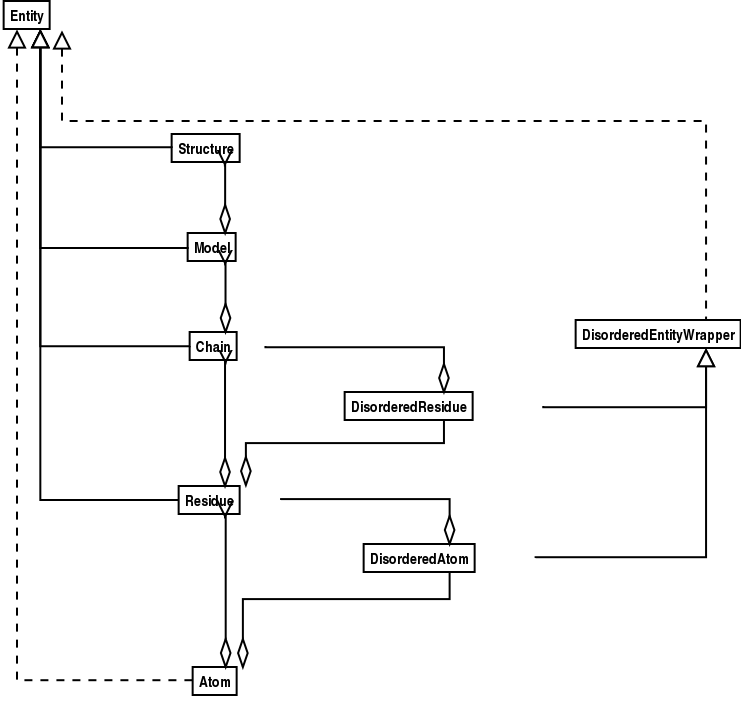
\includegraphics[width=0.8\textwidth]{images/smcra.png}
\label{fig:smcra}
\caption{UML diagram of the SMCRA data structure 
used to represent a macromolecular structure.}
\end{figure}
\end{latexonly}


Structure, Model, Chain and Residue are all subclasses of the Entity base class.
The Atom class only (partly) implements the Entity interface (because an Atom
does not have children). 

For each Entity subclass, you can extract a child by using a unique id for that
child as a key (e.g. you can extract an Atom object from a Residue object by
using an atom name string as a key, you can extract a Chain object from a Model
object by using its chain identifier as a key). 

Disordered atoms and residues are represented by DisorderedAtom and DisorderedResidue
classes, which are both subclasses of the DisorderedEntityWrapper base class.
They hide the complexity associated with disorder and behave exactly as Atom
and Residue objects. 

In general, a child Entity object (i.e. Atom, Residue, Chain, Model) can be
extracted from its parent (i.e. Residue, Chain, Model, Structure, respectively)
by using an id as a key.

\begin{verbatim}
child_entity=parent_entity[child_id]
\end{verbatim}

You can also get a list of all child Entities of a parent Entity object. Note
that this list is sorted in a specific way (e.g. according to chain identifier
for Chain objects in a Model object). 

\begin{verbatim}
child_list=parent_entity.get_list()
\end{verbatim}

You can also get the parent from a child.

\begin{verbatim}
parent_entity=child_entity.get_parent()
\end{verbatim}

At all levels of the SMCRA hierarchy, you can also extract a \emph{full id}.
The full id is a tuple containing all id's starting from the top object (Structure)
down to the current object. A full id for a Residue object e.g. is something
like: 

\begin{verbatim}
full_id=residue.get_full_id()

print full_id

("1abc", 0, "A", ("", 10, "A"))
\end{verbatim}

This corresponds to: 

\begin{itemize}
\item The Structure with id \char`\"{}1abc\char`\"{}
\item The Model with id 0 
\item The Chain with id \char`\"{}A\char`\"{}
\item The Residue with id (\char`\"{} \char`\"{}, 10, \char`\"{}A\char`\"{}). 
\end{itemize}
The Residue id indicates that the residue is not a hetero-residue (nor a water)
because it has a blanc hetero field, that its sequence identifier is 10 and
that its insertion code is \char`\"{}A\char`\"{}.

Some other useful methods:

\begin{verbatim}
# get the entity's id

entity.get_id()

# check if there is a child with a given id

entity.has_id(entity_id)

# get number of children

nr_children=len(entity)
\end{verbatim}

It is possible to delete, rename, add, etc. child entities from a parent entity,
but this does not include any sanity checks (e.g. it is possible to add two
residues with the same id to one chain). This really should be done via a nice
Decorator class that includes integrity checking, but you can take a look at
the code (Entity.py) if you want to use the raw interface. 

\subsubsection{Structure}

The Structure object is at the top of the hierarchy. Its id is a user given
string. The Structure contains a number of Model children. Most crystal structures
(but not all) contain a single model, while NMR structures typically consist
of several models. Disorder in crystal structures of large parts of molecules
can also result in several models. 

\paragraph{Constructing a Structure object}

A Structure object is produced by a PDBParser object:

\begin{verbatim}
from Bio.PDB.PDBParser import PDBParser

p=PDBParser(PERMISSIVE=1)

structure_id="1fat"

filename="pdb1fat.ent"

s=p.get_structure(structure_id, filename)
\end{verbatim}

The {\tt PERMISSIVE} flag indicates that a number of common problems (see \ref{problem structures})
associated with PDB files will be ignored (but note that some atoms and/or residues
will be missing). If the flag is not present a {\tt PDBConstructionException}
will be generated during the parse operation.

\paragraph{Header and trailer}

You can extract the header and trailer (simple lists of strings) of the PDB
file from the PDBParser object with the {\tt get\_header} and {\tt get\_trailer}
methods.


\subsubsection{Model}

The id of the Model object is an integer, which is derived from the position
of the model in the parsed file (they are automatically numbered starting from
0). The Model object stores a list of Chain children. 


\paragraph{Example}

Get the first model from a Structure object.

\begin{verbatim}
first_model=structure[0]
\end{verbatim}

\subsubsection{Chain}

The id of a Chain object is derived from the chain identifier in the structure
file, and can be any string. Each Chain in a Model object has a unique id. The
Chain object stores a list of Residue children. 


\paragraph{Example}

Get the Chain object with identifier {}``A{}'' from a Model object.

\begin{verbatim}
chain_A=model["A"]
\end{verbatim}

\subsubsection{Residue}

Unsurprisingly, a Residue object stores a set of Atom children. In addition,
it also contains a string that specifies the residue name (e.g. {}``ASN{}'')
and the segment identifier of the residue (well known to X-PLOR users, but not
used in the construction of the SMCRA data structure). 

The id of a Residue object is composed of three parts: the hetero field (hetfield),
the sequence identifier (resseq) and the insertion code (icode). 

The hetero field is a string : it is {}``W{}'' for waters, {}``H\_{}'' followed
by the residue name (e.g. {}``H\_FUC{}'') for other hetero residues and blank
for standard amino and nucleic acids. This scheme is adopted for reasons described
in section \ref{hetero probems}.

The second field in the Residue id is the sequence identifier, an integer describing
the position of the residue in the chain.

The third field is a string, consisting of the insertion code. The insertion
code is sometimes used to preserve a certain desirable residue numbering scheme.
A Ser 80 insertion mutant (inserted e.g. between a Thr 80 and an Asn 81 residue)
could e.g. have sequence identifiers and insertion codes as followed: Thr 80
A, Ser 80 B, Asn 81. In this way the residue numbering scheme stays in tune
with that of the wild type structure. 

Let's give some examples. Asn 10 with a blank insertion code would have residue
id {\tt ('' '', 10, '' '')}. Water 10 would have residue id {\tt (``W``, 10, `` ``)}.
A glucose molecule (a hetero residue with residue name GLC) with sequence identifier
10 would have residue id {\tt (''H\_GLC'', 10, '' '')}. In this way, the three
residues (with the same insertion code and sequence identifier) can be part
of the same chain because their residue id's are distinct.

In most cases, the hetflag and insertion code fields will be blank, e.g. {\tt ('' '', 10, '' '')}.
In these cases, the sequence identifier can be used as a shortcut for the full
id:

\begin{verbatim}
# use full id

res10=chain[("", 10, "")]

# use shortcut 

res10=chain[10]
\end{verbatim}

Each Residue object in a Chain object should have a unique id. However, disordered
residues are dealt with in a special way, as described in section \ref{point mutations}.

A Residue object has a number of additional methods:

\begin{verbatim}
r.get_resname()		# return residue name, e.g. "ASN"
r.get_segid()		# return the SEGID, e.g. "CHN1"
\end{verbatim}

\subsubsection{Atom}

The Atom object stores the data associated with an atom, and has no children.
The id of an atom is its atom name (e.g. {}``OG{}'' for the side chain oxygen
of a Ser residue). An Atom id needs to be unique in a Residue. Again, an exception
is made for disordered atoms, as described in section \ref{disordered atoms}.

In a PDB file, an atom name consists of 4 chars, typically with leading and
trailing spaces. Often these spaces can be removed for ease of use (e.g. an
amino acid C\( \alpha  \) atom is labeled {}``.CA.{}'' in a PDB file, where
the dots represent spaces). To generate an atom name (and thus an atom id) the
spaces are removed, unless this would result in a name collision in a Residue
(i.e. two Atom objects with the same atom name and id). In the latter case,
the atom name including spaces is tried. This situation can e.g. happen when
one residue contains atoms with names {}``.CA.{}'' and {}``CA..{}'', although
this is not very likely. 

The atomic data stored includes the atom name, the atomic coordinates (including
standard deviation if present), the B factor (including anisotropic B factors
and standard deviation if present), the altloc specifier and the full atom name
including spaces. Less used items like the atom element number or the atomic
charge sometimes specified in a PDB file are not stored. 

An Atom object has the following additional methods: 

\begin{verbatim}
a.get_name()       # atom name (spaces stripped, e.g. "CA")

a.get_id()         # id (equals atom name)

a.get_coord()      # atomic coordinates

a.get_bfactor()    # B factor

a.get_occupancy()  # occupancy

a.get_altloc()     # alternative location specifie

a.get_sigatm()     # std. dev. of atomic parameters

a.get_siguij()     # std. dev. of anisotropic B factor

a.get_anisou()     # anisotropic B factor

a.get_fullname()   # atom name (with spaces, e.g. ".CA.")
\end{verbatim}

To represent the atom coordinates, siguij, anisotropic B factor and sigatm Numpy
arrays are used.


\subsection{Disorder}


\subsubsection{General approach\label{disorder problems}}

Disorder should be dealt with from two points of view: the atom and the residue
points of view. In general, we have tried to encapsulate all the complexity that
arises from disorder. If you just want to loop over all C\( \alpha  \) atoms,
you do not care that some residues have a disordered side chain. On the other
hand it should also be possible to represent disorder completely in the data
structure. Therefore, disordered atoms or residues are stored in special objects
that behave as if there is no disorder. This is done by only representing a
subset of the disordered atoms or residues. Which subset is picked (e.g. which
of the two disordered OG side chain atom positions of a Ser residue is used)
can be specified by the user.


\subsubsection{Disordered atoms\label{disordered atoms}}

Disordered atoms are represented by ordinary Atom objects, but all Atom objects
that represent the same physical atom are stored in a DisorderedAtom object.
Each Atom object in a DisorderedAtom object can be uniquely indexed using its
altloc specifier. The DisorderedAtom object forwards all uncaught method calls
to the selected Atom object, by default the one that represents the atom with
with the highest occupancy. The user can of course change the selected Atom
object, making use of its altloc specifier. In this way atom disorder is represented
correctly without much additional complexity. In other words, if you are not
interested in atom disorder, you will not be bothered by it.

Each disordered atom has a characteristic altloc identifier. You can specify
that a DisorderedAtom object should behave like the Atom object associated with
a specific altloc identifier:

\begin{verbatim}
atom.disordered\_select("A")		# select altloc A atom

print atom.get_altloc()
"A"

atom.disordered_select("B")	   	# select altloc B atom
print atom.get_altloc()
"B"
\end{verbatim}

\subsubsection{Disordered residues}

\paragraph{Common case}

The most common case is a residue that contains one or more disordered atoms.
This is evidently solved by using DisorderedAtom objects to represent the disordered
atoms, and storing the DisorderedAtom object in a Residue object just like ordinary
Atom objects. The DisorderedAtom will behave exactly like an ordinary atom (in
fact the atom with the highest occupancy) by forwarding all uncaught method
calls to one of the Atom objects (the selected Atom object) it contains. 


\paragraph{Point mutations\label{point mutations}}

A special case arises when disorder is due to a point mutation, i.e. when two
or more point mutants of a polypeptide are present in the crystal. An example
of this can be found in PDB structure 1EN2. 

Since these residues belong to a different residue type (e.g. let's say Ser
60 and Cys 60) they should not be stored in a single Residue object as in the
common case. In this case, each residue is represented by one Residue object,
and both Residue objects are stored in a DisorderedResidue object. 

The DisorderedResidue object forwards all uncaught methods to the selected Residue
object (by default the last Residue object added), and thus behaves like an
ordinary residue. Each Residue object in a DisorderedResidue object can be uniquely
identified by its residue name. In the above example, residue Ser 60 would have
id {}``SER{}'' in the DisorderedResidue object, while residue Cys 60 would
have id {}``CYS{}''. The user can select the active Residue object in a DisorderedResidue
object via this id.


\subsection{Hetero residues}


\subsubsection{Associated problems\label{hetero probems}}

A common problem with hetero residues is that several hetero and non-hetero
residues present in the same chain share the same sequence identifier (and insertion
code). Therefore, to generate a unique id for each hetero residue, waters and
other hetero residues are treated in a different way. 

Remember that Residue object have the tuple (hetfield, resseq, icode) as id.
The hetfield is blank ({}`` {}``) for amino and nucleic acids, and a string
for waters and other hetero residues. The content of the hetfield is explained
below.

\subsubsection{Water residues}

The hetfield string of a water residue consists of the letter {}``W{}''. So
a typical residue id for a water is ({}``W{}'', 1, {}`` {}``).

\subsubsection{Other hetero residues}

The hetfield string for other hetero residues starts with {}``H\_{}'' followed
by the residue name. A glucose molecule e.g. with residue name {}``GLC{}''
would have hetfield {}``H\_GLC{}''. It's residue id could e.g. be ({}``H\_GLC{}'',
1, {}`` {}``).

\subsection{Some random usage examples}

Parse a PDB file, and extract some Model, Chain, Residue and Atom objects.

\begin{verbatim}
from PDBParser import PDBParser 

parser=PDBParser()

structure=parser.get_structure("test", "1fat.pdb")
model=structure[0]
chain=model["A"]
residue=chain[1]
atom=residue["CA"]
\end{verbatim}

Extract a hetero residue from a chain (e.g. a glucose (GLC) moiety with resseq
10).

\begin{verbatim}
residue_id=("H_GLC", 10, " ")
residue=chain[residue_id]
\end{verbatim}

Print all hetero residues in chain.

\begin{verbatim}
for residue in chain.get_list():
	residue_id=residue.get_id()
	hetfield=residue_id[0]
	if hetfield[0]=="H":
		print residue_id
\end{verbatim}

Print out the coordinates of all CA atoms in a structure with B factor greater
than 50. 

\begin{verbatim}
for model in structure.get_list():
  for chain in model.get_list():
    for residue in chain.get_list():
      if residue.has_id("CA"):
        ca=residue["CA"]
        if ca.get_bfactor()>50.0:
          print ca.get_coord()
\end{verbatim}

Print out all the residues that contain disordered atoms.

\begin{verbatim}
for model in structure.get_list()
  for chain in model.get_list():
    for residue in chain.get_list():
      if residue.is_disordered():
        resseq=residue.get_id()[1]
        resname=residue.get_resname()
        model_id=model.get_id()
        chain_id=chain.get_id()
        print model_id, chain_id, resname, resseq
\end{verbatim}

Loop over all disordered atoms, and select all atoms with altloc A (if present).
This will make sure that the SMCRA data structure will behave as if only the
atoms with altloc A are present. 

\begin{verbatim}
for model in structure.get_list()
  for chain in model.get_list():
    for residue in chain.get_list():
      if residue.is_disordered():
        for atom in residue.get_list():
          if atom.is_disordered():
            if atom.disordered_has_id("A"):
              atom.disordered_select("A")
\end{verbatim}

Suppose that a chain has a point mutation at position 10, consisting of a Ser
and a Cys residue. Make sure that residue 10 of this chain behaves as the Cys
residue.

\begin{verbatim}
residue=chain[10]
residue.disordered_select("CYS")
\end{verbatim}

\subsection{Common problems in PDB files}


\subsubsection{Examples\label{problem structures}}

The PDBParser/Structure class was tested on about 800 structures (each belonging
to a unique SCOP superfamily). This takes about 20 minutes, or on average 1.5
seconds per structure. Parsing the structure of the large ribosomal subunit
(1FKK), which contains about 64000 atoms, takes 10 seconds on a 1000 MHz PC.

Three exceptions were generated in cases where an unambiguous data structure
could not be built. In all three cases, the likely cause is an error in the
PDB file that should be corrected. Generating an exception in these cases 
is much better than running the chance of incorrectly describing
the structure in a data structure. 


\paragraph{Duplicate residues}

One structure contains two amino acid residues in one chain with the same sequence
identifier (resseq 3) and icode. Upon inspection it was found that this chain
contains the residues Thr A3, \ldots{}, Gly A202, Leu A3, Glu A204. Clearly,
Leu A3 should be Leu A203. A couple of similar situations exist for structure
1FFK (which e.g. contains Gly B64, Met B65, Glu B65, Thr B67, i.e. residue Glu
B65 should be Glu B66). 


\paragraph{Duplicate atoms}

Structure 1EJG contains a Ser/Pro point mutation in chain A at position 22.
In turn, Ser 22 contains some disordered atoms. As expected, all atoms belonging
to Ser 22 have a non-blank altloc specifier (B or C). All atoms of Pro 22 have
altloc A, except the N atom which has a blank altloc. This generates an exception,
because all atoms belonging to two residues at a point mutation should have
non-blank altloc. It turns out that this atom is probably shared by Ser and
Pro 22, as Ser 22 misses the N atom. Again, this points to a problem in the
file: the N atom should be present in both the Ser and the Pro residue, in both
cases associated with a suitable altloc identifier.


\subsubsection{Automatic correction}

Some errors are quite common and can be easily corrected without much risk of
making a wrong interpretation. These cases are listed below.


\paragraph{A blank altloc for a disordered atom}

Normally each disordered atom should have a non-blanc altloc identifier. However,
there are many structures that do not follow this convention, and have a blank
and a non-blank identifier for two disordered positions of the same atom. This
is automatically interpreted in the right way. 


\paragraph{Broken chains}

Sometimes a structure contains a list of residues belonging to chain A, followed
by residues belonging to chain B, and again followed by residues belonging to
chain A, i.e. the chains are {}``broken{}''. This is correctly interpreted.


\subsubsection{Fatal errors}

Sometimes a PDB file cannot be unambiguously interpreted. Rather than guessing
and risking a mistake, an exception is generated, and the user is expected to
correct the PDB file. These cases are listed below.


\paragraph{Duplicate residues}

All residues in a chain should have a unique id. This id is generated based
on:

\begin{itemize}
\item The sequence identifier (resseq).
\item The insertion code (icode).
\item The hetfield string ({}``W{}'' for waters and {}``H\_{}'' followed by the
residue name for other hetero residues) 
\item The residue names of the residues in the case of point mutations (to store the
Residue objects in a DisorderedResidue object).
\end{itemize}
If this does not lead to a unique id something is quite likely wrong, and an
exception is generated.


\paragraph{Duplicate atoms}

All atoms in a residue should have a unique id. This id is generated based on:

\begin{itemize}
\item The atom name (without spaces, or with spaces if a problem arises).
\item The altloc specifier.
\end{itemize}
If this does not lead to a unique id something is quite likely wrong, and an
exception is generated.

\subsection{Other features}

There are also some tools to analyze a crystal structure. Tools
exist to superimpose two coordinate sets (SVDSuperimposer), to extract 
polypeptides from a structure (Polypeptide), to perform neighbor lookup
(NeighborSearch) and to write out PDB files (PDBIO). The neighbor lookup
is done using a KD tree module written in C++. It is very fast and also
includes a fast method to find all point pairs within a certain distance 
of each other.

A Polypeptide object is simply a UserList of Residue objects. You can 
construct a list of Polypeptide objects from a Structure object as follows:

\begin{verbatim}
model_nr=1
polypeptide_list=build_peptides(structure, model_nr)

for polypeptide in polypeptide_list:
    print polypeptide
\end{verbatim}

The Polypeptide objects are always created from a single 
Model (in this case model 1).

\section{Miscellaneous}

\subsection{Translating a DNA sequence to Protein}

\chapter{Advanced}

\section{Sequence Class}

\section{Regression Testing Framework}
\label{sec:regr_test}

Biopython has a regression testing framework written Andrew Dalke and ported to PyUnit by Brad Chapman which helps us make sure the code is as bug-free as possible before going out.

\subsection{Writing a Regression Test}

Every module that goes into Biopython should have a test (and should also have documentation!). Let's say you've written a new module called Biospam -- here is what you should do to make a regression test:

\begin{enumerate}
  \item Write a script called \verb|test_Biospam.py|

  \begin{itemize}

    \item This script should live in the Tests directory
       
     \item The script should test all of the important functionality of the module (the more you test the better your test is, of course!).
  \end{itemize}
       
  \item If the script requires files to do the testing, these should go in
       the directory Tests/Biospam.
       
  \item Write out the test output and verify the output to be correct. 
       There are two ways to do this:

  \begin{enumerate}
    \item The long way:

    \begin{itemize}
       
     \item Run the script and write its output to a file. On UNIX machines,
       you would do something like: \verb|python test_Biospam.py > test_Biospam| which would write the output to the file \verb|test_Biospam|.
       
     \item Manually look at the file \verb|test_Biospam| to make sure the output is correct. When you are sure it is all right and there are no bugs, you need to quickly edit the \verb|test_Biospam| file so that the first line is: '\verb|test_Biospam|' (no quotes).

     \item copy the \verb|test_Biospam| file to the directory Tests/output
     
   \end{itemize}

   \item The quick way:

   \begin{itemize}
      \item Run \verb|python run_tests.py -g test_Biospam.py|. The
            regression testing framework is nifty enough that it'll put
            the output in the right place in just the way it likes it.   
       
       \item Go to the output (which should be in \verb|Tests/output/test_Biospam|) and double check the output to make sure it is all correct. 

   \end{itemize}

 \end{enumerate}
       
 \item Now change to the Tests directory and run the regression tests
       with \verb|python run_tests.py|. This will run all of the tests, and
       you should see your test run (and pass!).
       
  \item That's it! Now you've got a nice test for your module.
       Congratulations!
\end{enumerate}


\section{Parser Design}

\subsection{Design Overview}

Parsers are built around an event-oriented design that includes
Scanner and Consumer objects.


Scanners take input from a data source and analyze it line by line,
sending off an event whenever it recognizes some information in the
data.  For example, if the data includes information about an organism
name, the scanner may generate an \verb|organism_name| event whenever it
encounters a line containing the name.


Consumers are objects that receive the events generated by Scanners.
Following the previous example, the consumer receives the
\verb|organism_name| event, and the processes it in whatever manner
necessary in the current application.

\subsection{Events}

There are two types of events: info events that tag the location of
information within a data stream, and section events that mark
sections within a stream.  Info events are associated with specific
lines within the data, while section events are not.


Section event names must be in the format \verb|start_EVENTNAME| and
\verb|end_EVENTNAME| where \verb|EVENTNAME| is the name of the event.


For example, a FASTA-formatted sequence scanner may generate the
following events:
\begin{verbatim}
EVENT NAME      ORIGINAL INPUT
begin_sequence  
title           >gi|132871|sp|P19947|RL30_BACSU 50S RIBOSOMAL PROTEIN L30 (BL27
sequence        MAKLEITLKRSVIGRPEDQRVTVRTLGLKKTNQTVVHEDNAAIRGMINKVSHLVSVKEQ
end_sequence
begin_sequence
title           >gi|132679|sp|P19946|RL15_BACSU 50S RIBOSOMAL PROTEIN L15
sequence        MKLHELKPSEGSRKTRNRVGRGIGSGNGKTAGKGHKGQNARSGGGVRPGFEGGQMPLFQRLPK
sequence        RKEYAVVNLDKLNGFAEGTEVTPELLLETGVISKLNAGVKILGNGKLEKKLTVKANKFSASAK
sequence        GTAEVI
end_sequence
[...]
\end{verbatim}

(I cut the lines shorter so they'd look nicer in my editor).


The FASTA scanner generated the following events: \verb|title|, \verb|sequence|,
\verb|begin_sequence|, and \verb|end_sequence|.  Note that the \verb|begin_sequence|
and \verb|end_sequence| events are not associated with any line in the
original input.  They are used to delineate separate sequences within
the file.


The events a scanner can send must be specifically defined for each
data format.


\subsection{'noevent' EVENT}

A data file can contain lines that have no meaningful information,
such as blank lines.  By convention, a scanner should generate the
"noevent" event for these lines.




\subsection{Scanners}

\begin{verbatim}
class Scanner:
    def feed(self, handle, consumer):
        # Implementation
\end{verbatim}


Scanners should implement a method named 'feed' that takes a file
handle and a consumer.  The scanner should read data from the file
handle and generate appropriate events for the consumer.

\subsection{Consumers}

\begin{verbatim}
class Consumer:
    # event handlers
\end{verbatim}


Consumers contain methods that handle events.  The name of the method
is the event that it handles.  Info events are passed the line of the
data containing the information, and section events are passed
nothing.


You are free to ignore events that are not interesting for your
application.  You should just not implement methods for those events.


All consumers should be derived from the base Consumer class.


An example:


\begin{verbatim}
class FASTAConsumer(Consumer):
    def title(self, line):
        # do something with the title
    def sequence(self, line):
        # do something with the sequence
    def begin_sequence(self):
        # a new sequence starts
    def end_sequence(self):
        # a sequence ends
\end{verbatim}


\subsection{BLAST}

BLAST Scanners produce the following events:

\begin{verbatim}
header
    version
    reference
    query_info
    database_info

descriptions
    description_header
    round                         psi blast
    model_sequences               psi blast
    nonmodel_sequences            psi blast
    converged                     psi blast
    description
    no_hits

alignment
    multalign                     master-slave
    title                         pairwise
    length                        pairwise
  hsp
    score                         pairwise
    identities                    pairwise
    strand                        pairwise, blastn
    frame                         pairwise, blastx, tblastn, tblastx
    query                         pairwise
    align                         pairwise
    sbjct                         pairwise

database_report
    database
    posted_date
    num_letters_in_database
    num_sequences_in_database
    num_letters_searched          RESERVED.  Currently unused.  I've never
    num_sequences_searched        RESERVED.  seen it, but it's in blastool.c..
    ka_params
    gapped                        not blastp
    ka_params_gap                 gapped mode (not tblastx)

parameters
    matrix
    gap_penalties                 gapped mode (not tblastx)
    num_hits                      
    num_sequences                 
    num_extends                   
    num_good_extends              
    num_seqs_better_e
    hsps_no_gap                   gapped (not tblastx) and not blastn
    hsps_prelim_gapped            gapped (not tblastx) and not blastn
    hsps_prelim_gap_attempted     gapped (not tblastx) and not blastn
    hsps_gapped                   gapped (not tblastx) and not blastn
    query_length
    database_length
    effective_hsp_length
    effective_query_length
    effective_database_length
    effective_search_space
    effective_search_space_used
    frameshift                    blastx or tblastn or tblastx
    threshold
    window_size
    dropoff_1st_pass
    gap_x_dropoff
    gap_x_dropoff_final           gapped (not tblastx) and not blastn
    gap_trigger
    blast_cutoff
\end{verbatim}

\subsection{Enzyme}
The Enzyme Scanner produces the following events:
\begin{verbatim}
record
    identification
    description
    alternate_name
    catalytic_activity
    cofactor
    comment
    disease
    prosite_reference
    databank_reference
    terminator
\end{verbatim}

\subsection{Fasta}
The Fasta Scanner produces the following events:
\begin{verbatim}
sequence
    title
    sequence
\end{verbatim}


\subsection{Medline}
The Online Services Reference Manual documents the MEDLINE format at:
\ahrefurl{\url{http://www.nlm.nih.gov/pubs/osrm_nlm.html}}

The Medline scanner produces the following events:
\begin{verbatim}
record
    undefined
    abstract_author
    abstract
    address
    author
    call_number
    comments
    class_update_date
    country
    entry_date
    publication_date
    english_abstract
    entry_month
    gene_symbol
    identification
    issue_part_supplement
    issn
    journal_title_code
    language
    special_list
    last_revision_date
    mesh_heading
    mesh_tree_number
    major_revision_date
    no_author
    substance_name
    pagination
    personal_name_as_subject
    publication_type
    number_of_references
    cas_registry_number
    record_originator
    journal_subset
    subheadings
    secondary_source_id
    source
    title_abbreviation
    title
    transliterated_title
    unique_identifier
    volume_issue
    year
    pubmed_id
\end{verbatim}    

undefined is a special event that is called for every line with a
qualifier not defined in the specification.


\subsection{Prosite}
The Prosite scanner produces the following events:
\begin{verbatim}
copyrights
    copyright
record
    identification
    accession
    date
    description
    pattern
    matrix
    rule
    numerical_results
    comment
    database_reference
    pdb_reference
    documentation
    terminator
\end{verbatim}

The PRODOC scanner produces the following events:
\begin{verbatim}
record
    accession
    prosite_reference
    text
    reference
\end{verbatim}


\subsection{SWISS-PROT}
The SProt Scanner produces the following events:
\begin{verbatim}
record
    identification
    accession
    date
    description
    gene_name
    organism_species
    organelle
    organism_classification
    reference_number
    reference_position
    reference_comment
    reference_cross_reference
    reference_author
    reference_title
    reference_location
    comment
    database_cross_reference
    keyword
    feature_table
    sequence_header
    sequence_data
    terminator
\end{verbatim}


The KeyWList scanner produces the following events:
\begin{verbatim}
header
keywords
    keyword
footer
    copyright
\end{verbatim}

\section{Substitution Matrices}

\subsection{SubsMat}

This module provides a class and a few routines for generating substitution matrices, similar to BLOSUM or PAM matrices, but based on user-provided data.

Additionally, you may select a matrix from MatrixInfo.py, a collection of established substitution matrices.

\begin{verbatim}
class SeqMat(UserDict.UserDict)
\end{verbatim}

\begin{enumerate}
  \item Attributes

  \begin{enumerate}
    \item \verb|self.data|: a dictionary in the form of \verb|{(i1,j1):n1, (i1,j2):n2,...,(ik,jk):nk}| where i, j are alphabet letters, and n is a value.

    \item \verb|self.alphabet|: a class as defined in Bio.Alphabet

    \item \verb|self.ab_list|: a list of the alphabet's letters, sorted. Needed mainly for internal purposes

    \item \verb|self.sum_letters|: a dictionary. \verb|{i1: s1, i2: s2,...,in:sn}| where:
    \begin{enumerate}
      \item i: an alphabet letter; 
      \item s: sum of all values in a half-matrix for that letter; 
      \item n: number of letters in alphabet.
    \end{enumerate}
  \end{enumerate}

  \item Methods

  \begin{enumerate}

    \item 
\begin{verbatim} 
__init__(self,data=None,alphabet=None,
         mat_type=NOTYPE,mat_name='',build_later=0):
\end{verbatim}

    \begin{enumerate}

      \item \verb|data|: can be either a dictionary, or another SeqMat instance.
      \item \verb|alphabet|: a Bio.Alphabet instance. If not provided, construct an alphabet from data.

      \item \verb|mat_type|: type of matrix generated. One of the following:

      \begin{description}
        \item[NOTYPE]     No type defined
        \item[ACCREP]     Accepted Replacements Matrix
        \item[OBSFREQ]    Observed Frequency Matrix 
        \item[EXPFREQ]    Expsected Frequency Matrix
        \item[SUBS]       Substitution Matrix       
        \item[LO]         Log Odds Matrix
      \end{description}

      \verb|mat_type| is provided automatically by some of SubsMat's functions.

      \item \verb|mat_name|: matrix name, such as "BLOSUM62" or "PAM250"

      \item \verb|build_later|: default false. If true, user may supply only alphabet and empty dictionary, if intending to build the matrix later. this skips the sanity check of alphabet size vs. matrix size. 

    \end{enumerate}

    \item
\begin{verbatim}
entropy(self,obs_freq_mat)
\end{verbatim}

    \begin{enumerate}
      \item \verb|obs_freq_mat|: an observed frequency matrix. Returns the matrix's entropy, based on the frequency in  \verb|obs_freq_mat|. The matrix instance should be LO or SUBS.
    \end{enumerate}


    \item
\begin{verbatim}
letter_sum(self,letter)
\end{verbatim}

    Returns the sum of all values in the matrix, for the provided \verb|letter|

    \item
\begin{verbatim}
all_letters_sum(self)
\end{verbatim}
    
    Fills the  dictionary attribute \verb|self.sum_letters| with the sum of values for each letter in the matrix's alphabet.


    \item
\begin{verbatim}
print_mat(self,f,format="%4d",bottomformat="%4s",alphabet=None)
\end{verbatim}

    prints the matrix to file handle f. \verb|format| is the format field for the matrix values; \verb|bottomformat| is the format field for the bottom row, containing matrix letters. Example output for a 3-letter alphabet matrix:

\begin{verbatim}
A 23
B 12 34
C 7  22  27
  A   B   C
\end{verbatim}

    The \verb|alphabet| optional argument is a string of all characters in the alphabet. If supplied, the order of letters along the axes is taken from the string, rather than by alphabetical order.

  \end{enumerate}

\item Usage

   The following section is layed out in the order by which most people wish to generate a log-odds matrix. Of course, interim matrices can be generated and
   investigated. Most people just want a log-odds matrix, that's all. 
   
   \begin{enumerate}

   \item Generating an Accepted Replacement Matrix

   Initially, you should generate an accepted replacement matrix (ARM) from your data. The values in ARM are the counted number of replacements according to your data. The data could be a set of pairs or multiple alignments. So for instance if Alanine was replaced by Cysteine 10 times, and Cysteine by Alanine 12 times, the corresponding ARM entries would be: 

\begin{verbatim}
('A','C'): 10, ('C','A'): 12 
\end{verbatim}

as order doesn't matter, user can already provide only one entry: 

\begin{verbatim}
('A','C'): 22 
\end{verbatim}

 A SeqMat instance may be initialized with either a full (first method of counting: 10, 12) or half (the latter method, 22) matrices. A full protein
   alphabet matrix would be of the size 20x20 = 400. A half matrix of that alphabet would be 20x20/2 + 20/2 = 210. That is because same-letter entries don't
   change. (The matrix diagonal). Given an alphabet size of N: 

   \begin{enumerate}
     \item Full matrix size:N*N 

     \item Half matrix size: N(N+1)/2 
   \end{enumerate}

The SeqMat constructor automatically generates a half-matrix, if a full matrix is passed. If a half matrix is passed, letters in the key should be provided in alphabetical order: ('A','C') and not ('C',A'). 

At this point, if all you wish to do is generate a log-odds matrix, please go to the section titled Example of Use. The following text describes the nitty-gritty of internal functions, to be used by people who wish to investigate their nucleotide/amino-acid frequency data more thoroughly. 

\item Generating the observed frequency matrix (OFM)

Use:
\begin{verbatim}
OFM = SubsMat._build_obs_freq_mat(ARM)
\end{verbatim}

  The OFM is generated from the ARM, only instead of replacement counts, it contains replacement frequencies. 

\item Generating an expected frequency matrix (EFM)

Use:

\begin{verbatim}
EFM = SubsMat._build_exp_freq_mat(OFM,exp_freq_table)
\end{verbatim}

  \begin{enumerate}
    \item \verb|exp_freq_table|: should be a FreqTable instance. See section~\ref{sec:freq_table} for detailed information on FreqTable. Briefly, the expected frequency table has the frequencies of appearance for each member of the alphabet. It is
  implemented as a dictionary with the alphabet letters as keys, and each letter's frequency as a value. Values sum to 1.
  \end{enumerate}
 
The expected frequency table can (and generally should) be generated from the observed frequency matrix. So in most cases you will generate \verb|exp_freq_table| using:

\begin{verbatim}
>>> exp_freq_table = SubsMat._exp_freq_table_from_obs_freq(OFM)
>>> EFM = SubsMat._build_exp_freq_mat(OFM,exp_freq_table)
\end{verbatim}

But you can supply your own \verb|exp_freq_table|, if you wish

\item Generating a substitution frequency matrix (SFM)

Use:

\begin{verbatim}
SFM = SubsMat._build_subs_mat(OFM,EFM)
\end{verbatim}

  Accepts an OFM, EFM. Provides the division product of the corresponding values. 

\item Generating a log-odds matrix (LOM)

   Use: 
\begin{verbatim}
LOM=SubsMat._build_log_odds_mat(SFM[,logbase=10,factor=10.0,round_digit=1])
\end{verbatim}

   \begin{enumerate}
     \item Accepts an SFM. 

     \item \verb|logbase|: base of the logarithm used to generate the log-odds values. 

     \item \verb|factor|: factor used to multiply the log-odds values.  Each entry is generated by log(LOM[key])*factor And rounded to the \verb|round_digit| place after the decimal point, if required.

\end{enumerate}

\end{enumerate}

\item Example of use

As most people would want to generate a log-odds matrix, with minimum hassle, SubsMat provides one function which does it all:


\begin{verbatim} 
make_log_odds_matrix(acc_rep_mat,exp_freq_table=None,logbase=10,
                      factor=10.0,round_digit=0):
\end{verbatim}

\begin{enumerate}
  \item \verb|acc_rep_mat|: user provided accepted replacements matrix
  \item \verb|exp_freq_table|: expected frequencies table. Used if provided, if not, generated from the \verb|acc_rep_mat|.
  \item \verb|logbase|: base of logarithm for the log-odds matrix. Default base 10.
  \item \verb|round_digit|: number after decimal digit to which result should be rounded. Default zero.
\end{enumerate}

\end{enumerate}

\subsection{FreqTable}
\label{sec:freq_table}

\begin{verbatim}
FreqTable.FreqTable(UserDict.UserDict)
\end{verbatim}

\begin{enumerate}

  \item Attributes:
  
  \begin{enumerate}
    \item \verb|alphabet|: A Bio.Alphabet instance.

    \item \verb|data|: frequency dictionary

    \item \verb|count|: count dictionary (in case counts are provided).
  \end{enumerate}
  


  \item Functions:
  
  \begin{enumerate}
    \item \verb|read_count(f)|: read a count file from stream f. Then convert to frequencies

    \item \verb|read_freq(f)|: read a frequency data file from stream f. Of course, we then don't have the counts, but it is usually the letter frquencies which are interesting.

  \end{enumerate}

  \item Example of use:

  The expected count of the residues in the database is sitting in a file, whitespace delimited, in the following format (example given for a 3-letter alphabet):

\begin{verbatim}
A   35
B   65
C   100
\end{verbatim}

And will be read using the \verb|FreqTable.read_count(file_handle)| function. 

An equivalent frequency file:

\begin{verbatim}
A  0.175
B  0.325
C  0.5 
\end{verbatim}

Conversely, the residue frequencies or counts can be passed as a dictionary. 
Example of a count dictionary (3-letter alphabet):

\begin{verbatim}
{'A': 35, 'B': 65, 'C': 100}
\end{verbatim}

Which means that an expected data count would give a 0.5 frequency 
for 'C', a 0.325 probability of 'B' and a 0.175 probability of 'A' 
out of 200 total, sum of A, B and C)
 
 A frequency dictionary for the same data would be:

\begin{verbatim}
{'A': 0.175, 'B': 0.325, 'C': 0.5}
\end{verbatim}

Summing up to 1.

When passing a dictionary as an argument, you should indicate whether it is a count or a frequency dictionary. Therefore the FreqTable class constructor requires two arguments: the dictionary itself, and FreqTable.COUNT or FreqTable.FREQ indicating counts or frequencies, respectively.


Read expected counts. readCount will already generate the frequencies
Any one of the following may be done to geerate the frequency table (ftab):

\begin{verbatim}
>>> from SubsMat import *
>>> ftab = FreqTable.FreqTable(my_frequency_dictionary,FreqTable.FREQ)
>>> ftab = FreqTable.FreqTable(my_count_dictionary,FreqTable.COUNT)
>>> ftab = FreqTable.read_count(open('myCountFile'))
>>> ftab = FreqTable.read_frequency(open('myFrequencyFile'))
\end{verbatim}

\end{enumerate}


\chapter{Where to go from here -- contributing to Biopython}

\section{Maintaining a distribution for a platform}
\label{sec:maintain_dist}

We try to release Biopython to make it as easy to install as possible for users. Thus, we try to provide the Biopython libraries in as many install formats as we can. Doing this from release to release can be a lot of work for developers, and sometimes requires them to maintain packages they are not all that familiar with. This section is meant to provide tips to encourage other people besides developers to maintain platform builds.


In general, this is fairly easy -- all you would need to do is produce the system specific package whenever we make a release. You should then check the package (of course!) to make sure it installs everything properly. Then you just send it to one of the main developers, they stick the package on the web site and just like that, you've contributed to Biopython! Snazzy.


Below are some tips for certain platforms to maybe get people started with helping out:

\begin{description}
  \item[RPMs] -- RPMs are pretty popular package systems on some platforms. There is lots of documentation on RPMs available at \ahrefurl{\url{http://www.rpm.org}} to help you get started with them. To create an RPM for your platform is really easy. You just need to be able to build the package from source (having a C compiler that works is thus essential) -- see the Biopython installation instructions for more info on this.


To make the RPM, you just need to do:

\begin{verbatim}
python setup.py bdist_rpm
\end{verbatim}

This will create an RPM for your specific platform and a source RPM in the directory \verb|dist|. This RPM should be good and ready to go, so this is all you need to do! Nice and easy.

\item[Windows] -- Windows products typically have a nice graphical installer that installs all of the essential components in the right place. We can use Disttutils to create a installer of this type fairly easily.


You must first make sure you have a C compiler on your Windows computer, and that you can compile and install things (see the Biopython installation instructions for info on how to do this).


Once you are setup with a C compiler, making the installer just requires doing:

\begin{verbatim}
python setup.py bdist_wininst
\end{verbatim}

Now you've got a Windows installer. Congrats!

\item[Macintosh] -- We would love to find someone who wants to maintain a Macintosh distribution, and make it available in a Macintosh friendly format like bin-hex. This would basically include finding a way to compile everything on the Mac, making sure all of the code written by us UNIX-based developers works well on the Mac, and providing any Mac-friendly hints for us.

\end{description}

Once you've got a package, please test it on your system to make sure it installs everything in a good way and seems to work properly. Once you feel good about it, send it off to one of the biopython developers (write to our main list serve at biopython@biopython.org if you're not sure who to send it to) and you've done it. Thanks!

\section{Bug Reports + Feature Requests}

Getting feedback on the Biopython modules is very important to us. Open-source projects like this benefit greatly from feedback, bug-reports (and patches!) from a wide variety of contributors.


The main forums for discussing feature requests and potential bugs are the biopython development lists:

\begin{itemize}
  \item \mailto{biopython@biopython.org} -- An unmoderated list for discussion of anything to do with biopython.

  \item \mailto{biopython-dev@biopython.org} -- A more development oriented list that is mainly used by developers (but anyone is free to contribute!).
\end{itemize}

Additionally, if you think you've found a bug, you can submit it to our
bug-tracking page at \ahrefurl{\url{http://bugzilla.open-bio.org/}}. This 
way, it won't get buried in anyone's Inbox and forgotten about.

\section{Contributing Code}

There are no barriers to joining biopython code development other than an interest in creating biology-related code in python. The best place to express an interest is on the biopython mailing lists -- just let us know you are interested in coding and what kind of stuff you want to work on. Normally, we try to have some discussion on modules before coding them, since that helps generate good ideas -- then just feel free to jump right in and start coding!


The main biopython release tries to be fairly uniform and interworkable,
to make it easier for users. You can read about some of (fairly
informal) coding style guidelines we try to use in biopython in the
contributing documentation at 
\ahrefurl{\url{http://www.biopython.org/docs/developer/contrib.html}}. We also try to add code to the distribution along with tests (see section~\ref{sec:regr_test} for more info on the regression testing framework) and documentation, so that everything can stay as workable and well documented as possible. This is, of course, the most ideal situation, under many situations you'll be able to find other people on the list who will be willing to help add documentation or more tests for your code once you make it available. So, to end this paragraph like the last, feel free to start working!


Additionally, if you have code that you don't think fits in the
distribution, but that you want to make available, we maintain Script
Central (\ahrefurl{\url{http://www.biopython.org/scriptcentral/}}) 
which has pointers to freely available code in python for bioinformatics.


Hopefully this documentation has got you excited enough about
biopython to try it out (and most importantly, contribute!). Thanks
for reading all the way through!

\chapter{Appendix: Useful stuff about Python}
\label{sec:appendix}

If you haven't spent a lot of time programming in python, many
questions and problems that come up in using Biopython are often
related to python itself. This section tries to present some ideas and 
code that come up often (at least for us!) while using the Biopython
libraries. If you have any suggestions for useful pointers that could
go here, please contribute!

\section{What the heck in a handle?}
\label{sec:appendix-handles}

Handles are mentioned quite frequently throughout this documentation,
and are also fairly confusing (at least to me!). Basically, you can
think of a handle as being a ``wrapper'' around text information.


Handles provide (at least) two benefits over plain text information:

\begin{enumerate}
  \item They provide a standard way to deal with information stored in 
  different ways. The text information can be in a file, or in a
  string stored in memory, or at some remote website, but the handle
  provides a common way of dealing with information in all of these
  formats. 

  \item They allow text information to be read incrementally, instead
  of all at once. This is really important when you are dealing with
  huge text files which would use up all of your memory if you had to
  load them all.
\end{enumerate}

Handles can deal with text information that is being read (i.~e.~reading 
from a file) or written (i.~e.~writing information to a file). In the
case of a ``read'' handle, commonly used functions are \verb|read()|,
which reads the entire text information from the handle, and
\verb|readline()|, which reads information one line at a time. For
``write'' handles, the function \verb|write()| is regularly used.


The most common usage for handles is reading information from a file,
which is done using the built-in python function \verb|open|:

\begin{verbatim}
>>> handle = open("m_cold.fasta", "r")
>>> handle.readline()
">gi|8332116|gb|BE037100.1|BE037100 MP14H09 MP Mesembryanthemum crystallinum cDNA 5' similar to cold acclimation protein, mRNA sequence\n"
\end{verbatim}

Handles are regularly used in Biopython for passing information to parsers.

\subsection{Creating a handle from a string}

One useful thing is to be able to turn information contained in a
string into a handle. The following example shows how to do this using 
\verb|cStringIO| from the Python standard library:

\begin{verbatim}
>>> my_info = 'A string\n with multiple lines.'
>>> print my_info
A string
 with multiple lines.
>>> import cStringIO
>>> my_info_handle = cStringIO.StringIO(my_info)
>>> first_line = my_info_handle.readline()
>>> print first_line
A string

>>> second_line = my_info_handle.readline()
>>> print second_line
 with multiple lines.
\end{verbatim}

\end{document}
